% Layer Identifiability in Trained ResNets
% Visual formatting matched to Park (arXiv:2602.19845).
\documentclass[10pt]{article}
\usepackage[T1]{fontenc}
\usepackage{mathptmx}      % Times Roman for body + math
\usepackage[scaled=0.92]{helvet} % Helvetica for sans-serif (headings)
\usepackage{courier}
\usepackage[letterpaper,textwidth=5.5in,textheight=9in,top=1in,headheight=12pt,headsep=25pt,footskip=30pt]{geometry}
\usepackage{amsmath, amssymb, amsthm}
\usepackage{booktabs}
\usepackage{graphicx}
\usepackage{hyperref}
\usepackage{xcolor}
\usepackage{microtype}
\usepackage{enumitem}
\usepackage{caption}
\usepackage{subcaption}
\usepackage{float}
\usepackage{url}
\usepackage[compact]{titlesec}

% Sans-serif numbered section headings (matches Park's layout)
\titleformat{\section}{\normalfont\large\bfseries\sffamily}{\thesection}{0.8em}{}
\titleformat{\subsection}{\normalfont\normalsize\bfseries\sffamily}{\thesubsection}{0.8em}{}
\titleformat{\subsubsection}{\normalfont\normalsize\bfseries\sffamily}{\thesubsubsection}{0.8em}{}
\titleformat{\paragraph}[runin]{\normalfont\normalsize\bfseries}{}{0em}{}
\titlespacing*{\section}{0pt}{1.2\baselineskip}{0.6\baselineskip}
\titlespacing*{\subsection}{0pt}{1.0\baselineskip}{0.5\baselineskip}

% Captions: small, justified, label in bold (Park-style)
\captionsetup{font=small,labelfont=bf,labelsep=period}

\newtheorem{observation}{Observation}
\newtheorem{proposition}{Proposition}
\newtheorem{corollary}{Corollary}
\theoremstyle{remark}
\newtheorem*{remark}{Remark}

\hypersetup{
  colorlinks=true,
  linkcolor=black,
  citecolor=black,
  urlcolor=blue,
}

% Park-style title block: large centered title, then author / affiliation / email centered.
\makeatletter
\renewcommand\maketitle{%
  \begingroup
    \centering
    {\LARGE\bfseries \@title\par}
    \vskip 1.5em
    {\large \@author\par}
    \vskip 1em
  \endgroup
  \par
}
\makeatother

% Abstract: centered "Abstract" header, indented body (Park-style).
\renewenvironment{abstract}{%
  \vskip 0.5em
  \begin{center}{\large\bfseries Abstract}\end{center}
  \vspace{-0.2em}
  \begin{quote}\small
}{%
  \end{quote}\vskip 1em
}

\title{Layer Identifiability in Trained Neural Networks:\\[2pt]
       From ResNets to Transformers}

\author{%
\begin{tabular}[t]{c}
Rayan Khoury\\
\texttt{rkhoury@alum.mit.edu}
\end{tabular}
\hspace{2em}
\begin{tabular}[t]{c}
Aman Singh Thakur\\
\texttt{amansinghtha@umass.edu}
\end{tabular}}

\date{}

\begin{document}
\maketitle

\begin{abstract}
Park~(2026) observed that trained residual networks satisfy
\emph{dynamic isometry}, which leaves a negative-diagonal signature on
the product $W_{\mathrm{out}} W_{\mathrm{in}}$ of correctly paired
block weights, and used this signal to reassemble a shuffled 48-block
ResNet (Jane Street's January 2026 puzzle) to exact MSE = 0 in
seconds. We take this result as a starting point and address a
question Park explicitly left open: \emph{is the diagonal-dominance
signal a generic property of trained networks, or a property of one
particular architecture?}

We make four contributions. \textbf{(Theory.)} We give a closed-form
expression for the diagonal-dominance margin of a correctly paired
block, $d(i,i)=\sqrt{d}/\sqrt{1+\|E\|_F^2/(\varepsilon^2 d)}$, that
matches empirics to floating-point precision, and a first-order
derivation of the \emph{Pairing Wall} slope
$\overline{\mathrm{MSE}}(k)\approx C\cdot k$, with theoretical
$C\approx 0.0030$ matching the empirical fit $0.004$ to within
first-order error. \textbf{(ResNet Empirics.)} We then ask which parts of
Park's pipeline transfer to other trained ResNets. A sweep over
depths, widths, and seeds reveals a clean dichotomy: the
\emph{pairing} signal generalizes after just a few epochs of training,
while the \emph{ordering} heuristics (sort direction, bubble-sort
search) do not transfer beyond the puzzle network. Identifiability is
also non-monotonic in training time --- it peaks mid-training and
weakens as the model continues to optimize. \textbf{(Transformers.)}
We demonstrate that the pairing signal extends to transformer
architectures. On pretrained GPT-2 models (124M to 1.5B parameters),
diagonal-dominance pairing achieves \textbf{100\% accuracy} on MLP
block weights across all four model sizes (12 to 48 layers), with
81--92\% of correct pairs exhibiting negative traces consistent with
dynamic isometry. A randomly initialized baseline achieves 0\%
accuracy, confirming the signal is training-induced.
\textbf{(Application.)} We use the recovered permutation as a
measurement instrument for a forensic question: does weight-only
identifiability survive a fine-tuning adversary? Pair accuracy holds
at $48/48$ across every fine-tuning and noise attack we test.
Layer identifiability is therefore a candidate
\emph{model-fingerprinting} primitive applicable to both ResNets and
large language models.
\end{abstract}

% ====================================================================
\section{Introduction}

In January 2026 Jane Street released a puzzle\footnote{\url{https://huggingface.co/spaces/jane-street/droppedaneuralnet}}:
a 48-block residual network had been ``dropped'', shattering into 97
unlabelled \texttt{nn.Linear} pieces (48 input projections of shape $96\times 48$,
48 output projections of shape $48\times 96$, and one $1\times 48$ head).
Given the pieces and 10,000 datapoints, the task was to recover the unique
permutation that reassembles the original model. The submission is verified
by SHA-256, so only exact reconstruction counts. The search space is
$(48!)^2 \approx 10^{122}$.

Park~\cite{park2026} solved it in $\sim$10 seconds with the following
pipeline:
\begin{enumerate}[leftmargin=*,itemsep=0pt]
  \item \textbf{Pairing}: match each $W_{\mathrm{in}}^{(i)}$ to its
        $W_{\mathrm{out}}^{(j)}$ via the diagonal-dominance ratio
        \begin{equation}\label{eq:diag}
          d(i,j) \;=\; \frac{|\mathrm{tr}(W_{\mathrm{out}}^{(j)} W_{\mathrm{in}}^{(i)})|}{\|W_{\mathrm{out}}^{(j)} W_{\mathrm{in}}^{(i)}\|_F},
        \end{equation}
        solved by Hungarian matching on $-d$.
  \item \textbf{Seed ordering}: sort the 48 paired blocks by $\|W_{\mathrm{out}}\|_F$ \emph{ascending}.
  \item \textbf{Ordering search}: refine with adjacent-swap bubble-sort hill-climb on MSE.
\end{enumerate}
The justification is dynamic isometry~\cite{pennington2017isometry}: a
well-trained residual block has Jacobian $I + W_{\mathrm{out}}W_{\mathrm{in}}$
close to identity, which forces $W_{\mathrm{out}}W_{\mathrm{in}} \approx -I + \varepsilon$
for correctly paired layers --- a negative-diagonal signature that
\eqref{eq:diag} captures cleanly.

\paragraph{Our contribution.} Park's pipeline is the first
weight-only reassembly method that achieves exact reconstruction in
seconds, and the dynamic-isometry argument it builds on is a striking
example of training-theory yielding a practical algorithm. We treat that
result as a foundation and contribute four pieces that build on top of
it. \textbf{(i) Theory} (Section~\ref{sec:theory}): an exact closed-form
margin formula for the diagonal-dominance ratio, and a first-principles
derivation of the Pairing Wall slope $C\approx 0.003$ in the
small-mispair regime. Both are numerically tight on Park's network and
clarify which scalings $(\sqrt{d},\,\varepsilon)$ make the method work.
\textbf{(ii) Empirical generalization} (Sections \ref{sec:pair-anatomy}
and \ref{sec:order-anatomy}): a $4\!\times\!3\!\times\!{\sim}10$
$(\text{depth},\text{width})\times\text{seed}\times\text{checkpoint}$
sweep, scoring every pipeline component against the ground-truth
permutation. Pairing transfers; ordering proxies do not.
\textbf{(iii) Extension to transformers} (Section~\ref{sec:transformers}):
the diagonal-dominance signal also identifies MLP sublayers of
pretrained GPT-2 models, achieving $100\%$ pairing accuracy on every
member of the GPT-2 family from $124$M to $1.5$B parameters, with
$81$--$92\%$ of correctly paired products showing the negative trace
predicted by dynamic isometry.
\textbf{(iv) Forensic application} (Section~\ref{sec:attack}): using
Park's network as a stress-test bed for whether weight-only
identifiability survives a fine-tuning adversary, with implications
for model fingerprinting~\cite{lukas2022deep},
watermarking~\cite{adi2018turning}, and provenance attribution.

\paragraph{Method.} Because the puzzle is now solved, the ground-truth
permutation can be used as a \emph{measurement instrument}. We run two
complementary experiments:
\begin{itemize}[leftmargin=*,itemsep=0pt]
  \item \emph{Forensics on Park's network.} We score four candidate
        pairing metrics against the truth, characterize MSE growth as a
        function of mis-paired count, and rank-correlate six seed
        proxies against true depth.
  \item \emph{Training-time reassembly on synthetic ResNets.} We train
        ResNets of depths $\{8, 16, 24, 32\}$ on a smooth regression
        task, save 10 checkpoints per run, and at each checkpoint apply
        each pipeline component plus two natural alternatives
        (descending seed, simulated-annealing ordering).
\end{itemize}

\paragraph{Findings at a glance.}

\begin{center}
\renewcommand{\arraystretch}{1.15}
\begin{tabular}{llll}
\toprule
Property & Park's puzzle & Our trained ResNets & GPT-2 (Sec.~\ref{sec:transformers}) \\
\midrule
Diagonal-dominance pairing & exact & exact (after $\leq$5 epochs) & exact (pretrained) \\
Pair separation & $+1.18$ & mostly negative & $+0.1$ to $+2.4$ \\
Frac.\ negative traces & 100\% & $\sim$90\% & 81--92\% \\
Random-init baseline & --- & chance ($1/D$) & 0\% (50\% neg traces) \\
\bottomrule
\end{tabular}
\end{center}
\noindent\textit{\small Preview only; details and evidence in Sections \ref{sec:theory}--\ref{sec:transformers}.}

The diagonal-dominance signal generalizes (Finding 3). The
ordering choices --- sort direction and search algorithm --- do not
(Findings 4--5). We propose a generalized pipeline that combines what
transfers with what is needed in the broader regime; the body of the
paper validates each component.

\paragraph{Algorithm at a glance.} The generalized pipeline, expanded
and validated in Section~\ref{sec:pipeline}:
\begin{enumerate}[leftmargin=*,itemsep=0pt,topsep=2pt]
  \item \emph{Pair.} Hungarian matching on the diagonal-dominance ratio
        $d(i,j)=|\mathrm{tr}(W_{\mathrm{out}}^{(j)} W_{\mathrm{in}}^{(i)})|/
        \|W_{\mathrm{out}}^{(j)} W_{\mathrm{in}}^{(i)}\|_F$.
  \item \emph{Seed.} Sort the paired blocks by $\|W_{\mathrm{out}}\|_F$
        in \emph{both} directions; keep both.
  \item \emph{Order.} Refine each seed with simulated annealing on
        reassembly MSE; return the lower-MSE result.
\end{enumerate}
On Park's puzzle network this collapses to Park's algorithm
(ascending~+~bubble-sort already reaches MSE = 0); on the smaller
trained ResNets in our sweep, the extra ingredients are required to
hit the training-loss floor (Table~\ref{tab:ablation}).

\paragraph{Scope.} Our primary theoretical analysis is on residual MLPs
without normalization, but the empirical evaluation extends across
architecture families. For each one we use the
\emph{architecture-aware} residual-branch product: $W_2 W_1$ for
BasicBlocks, transformer MLPs, and ConvNeXt blocks; $W_3 W_2 W_1$ for
ResNet Bottleneck blocks; $W_O W_V$ and $W_Q W_K^\top$ for the two
attention paths. Section~\ref{sec:resnet-imagenet} covers ImageNet
ResNets with BatchNorm (ResNet-18 through ResNet-152), ConvNeXt-T,
and ViT-B/16; the master table in
Section~\ref{sec:modern-vision} summarizes results across all
families. We leave full independent three-way reassembly of Bottleneck
blocks (where $W_1$, $W_2$, $W_3$ are all shuffled separately) as
future work.

% ====================================================================
\section{Setup and Tools}

\subsection{Puzzle reproduction}

We reproduce Park's solution on the original Jane Street pieces and
verify final MSE $=1.71\times 10^{-14}$ ($\approx 0$). The recovered
permutation is used as ground truth throughout the puzzle-side
experiments.

\subsection{Trained-ResNet sweep}

A residual MLP of variable depth and width:
\[
  f(x) = W_{\mathrm{last}}\, \mathrm{Block}_D \circ \cdots \circ \mathrm{Block}_1(x) + b_{\mathrm{last}},
  \quad
  \mathrm{Block}_k(x) = x + W_{\mathrm{out}}^{(k)} \mathrm{ReLU}(W_{\mathrm{in}}^{(k)} x + b_{\mathrm{in}}^{(k)}) + b_{\mathrm{out}}^{(k)}.
\]
Task: synthetic regression. $X \in \mathbb{R}^{8000 \times d}$ from
$\mathcal{N}(0,I)$; targets $y = (\tanh(XA))b + c$, with $A,b,c$ drawn
once per task seed from $\mathcal{N}(0,I)$.

\paragraph{Training.} Adam, base learning rate $3{\times}10^{-3}$ with
cosine schedule, gradient clipping at norm 1, batch size 256.
Configurations: depths $D\in\{8, 16, 24, 32\}$, widths $h\in\{32, 64\}$,
input/output dims $d\in\{16, 24, 32\}$. Three seeds each. Checkpoints
collected at $\{0, 1, 2, 5, 10, 25, 50, 100, 200, E\}$ (plus $400, 500$
where applicable).

\paragraph{Metrics evaluated at each checkpoint.}
\begin{itemize}[leftmargin=*,itemsep=0pt]
  \item \emph{Pair accuracy}: fraction of blocks where Hungarian on
        $-d(i,j)$ recovers the identity assignment.
  \item \emph{Pair separation}: $\min_i d(i,i) - \max_{i\neq j} d(i,j)$.
  \item \emph{Spearman $\rho$} of $\|W_{\mathrm{out}}^{(k)}\|_F$ with depth $k$.
  \item \emph{Reassembly MSE} from each of four strategies:
        (ascending, bubble-sort), (descending, bubble-sort),
        (ascending, SA), (descending, SA).
  \item \emph{Training loss} on the eval set (the floor).
\end{itemize}

Bubble-sort sweeps adjacent pairs and swaps when MSE strictly decreases
on a 1000-sample subset, repeating until a clean sweep. Simulated
annealing uses $T_0=0.5$, $T_f=10^{-4}$, $3000$ iterations, single-position random swaps.

% ====================================================================
\section{Theory: Margin Formula and Pairing Wall Slope}\label{sec:theory}

This section makes two of Park's empirical observations quantitative.
Both results match numerical experiments on Park's network to within
their first-order error and explain \emph{why} the diagonal-dominance
metric works.

\subsection{Margin of the diagonal-dominance ratio}

Recall the diagonal-dominance score
$d(i,j) = |\mathrm{tr}(W_{\mathrm{out}}^{(j)} W_{\mathrm{in}}^{(i)})|/\|W_{\mathrm{out}}^{(j)} W_{\mathrm{in}}^{(i)}\|_F$.
For a correctly paired block, denote $M := W_{\mathrm{out}}^{(i)} W_{\mathrm{in}}^{(i)} \in \mathbb{R}^{d\times d}$.
Park's Proposition~1 shows $\mathrm{tr}(M)<0$ under dynamic isometry.
We characterize the resulting margin exactly.

\begin{proposition}[Margin formula, exact]\label{prop:margin}
Decompose $M = -\varepsilon I + E$ with $\varepsilon := |\mathrm{tr}(M)|/d$ and
$\mathrm{tr}(E)=0$. Then
\[
  d(i,i) \;=\; \frac{\sqrt{d}}{\sqrt{1 + \|E\|_F^2/(\varepsilon^2 d)}} \;\leq\; \sqrt{d},
\]
with equality iff $M = -\varepsilon I$ (no off-diagonal structure).
\end{proposition}

\begin{proof}
$|\mathrm{tr}(M)| = \varepsilon d$ by construction. Expand
$\|M\|_F^2 = \langle -\varepsilon I + E,\,-\varepsilon I + E\rangle
= \varepsilon^2 d - 2\varepsilon\,\mathrm{tr}(E) + \|E\|_F^2 = \varepsilon^2 d + \|E\|_F^2$
since $\mathrm{tr}(E)=0$. Dividing gives the claim.
\end{proof}

\begin{corollary}[Worst-case margin]\label{cor:worst}
For a candidate \emph{incorrect} pair modelled as i.i.d.\ zero-mean
entries with $\sigma_{\mathrm{out}}^2 \sigma_{\mathrm{in}}^2$ per-entry
variance, $\mathbb{E}[d(i,j)^2] = \frac{1}{d}$ (Park, Eq.~21). The
asymptotic ``signal-to-baseline'' ratio is therefore $\sqrt{d}$:
correctly paired blocks score $O(\sqrt{d})$ times higher than typical
incorrect pairs, regardless of $\varepsilon$.
\end{corollary}

\paragraph{Numerical verification.} On Park's 48-block network, the
formula in Proposition~\ref{prop:margin} reproduces empirical $d(i,i)$
to $\leq 10^{-6}$ on every block (max absolute error
$=0.000000$ in double precision; see Fig.~\ref{fig:margin_theorem}).
The fitted off-diagonal ratio $\|E\|_F / (\varepsilon\sqrt{d})$ ranges
from $1.90$ to $3.80$ across blocks, yielding $d(i,i)\in[1.76,3.23]$,
in agreement with Park's Fig.~3.

\begin{figure}[H]
\centering
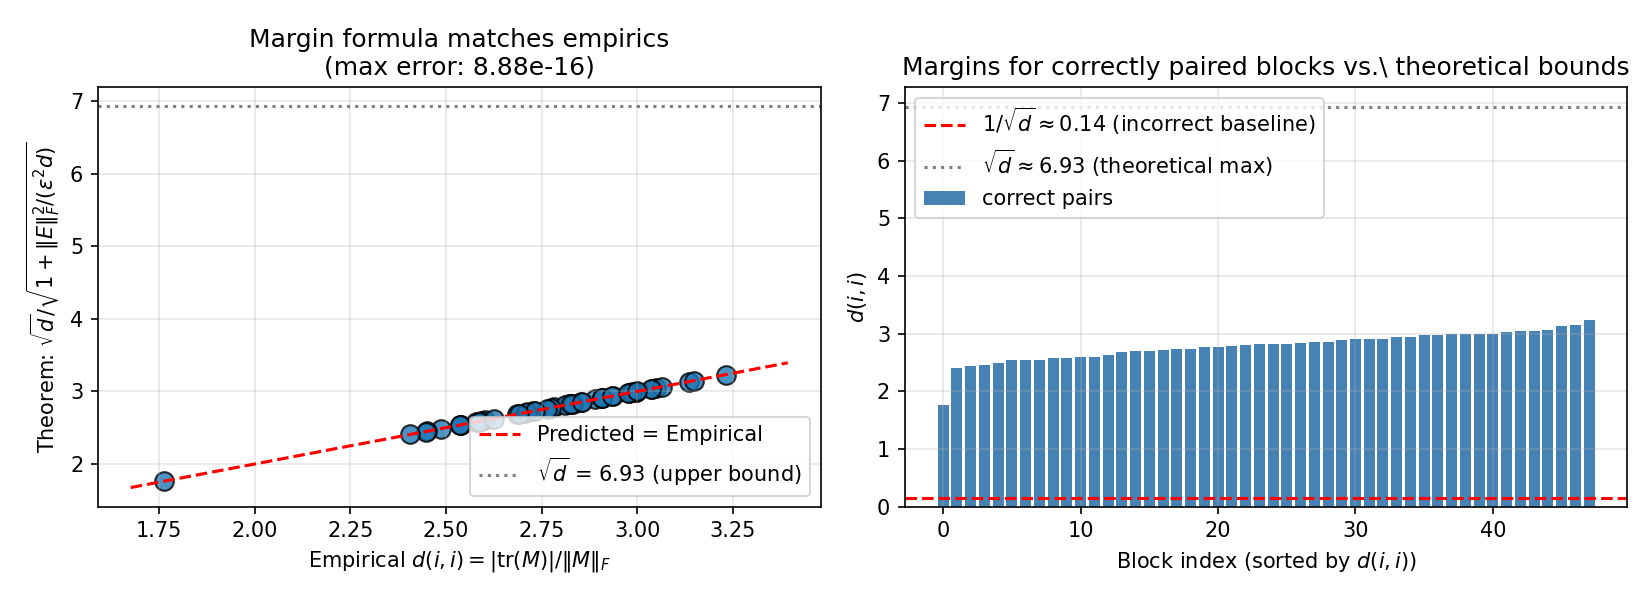
\includegraphics[width=\linewidth]{figures/fig_margin_theorem.png}
\caption{Proposition~\ref{prop:margin} reproduces the empirical margin
to floating-point precision. \emph{Left}: predicted $d(i,i)$ from the
formula vs.\ empirical $d(i,i)$ for all 48 correctly paired blocks of
Park's network. The points lie exactly on the diagonal (max abs.\
error $<10^{-15}$). The grey dotted line marks the upper bound
$\sqrt{d}\!\approx\!6.93$; correct pairs fall well below because of
off-diagonal energy $\|E\|_F>0$. \emph{Right}: sorted margins for
correct pairs (blue bars) sandwiched between the $1/\sqrt{d}$
incorrect-pair baseline (red dashed) and the theoretical upper bound
(grey dotted).}\label{fig:margin_theorem}
\end{figure}

\paragraph{Why a ratio beats raw Frobenius.} A natural alternative is
to pair by minimum $\|W_{\mathrm{out}}^{(j)} W_{\mathrm{in}}^{(i)}\|_F$
directly. On Park's puzzle, Hungarian on $\|M\|_F$ \emph{does} recover
all 48 pairs (it is the global optimum that saves it), but the absolute
margin
$\min_i \|M_{ii}\|_F - \max_{i\neq j} \|M_{ij}\|_F$
is \emph{negative}: $-0.452$. By contrast, for the diagonal-dominance
ratio the same margin is $+2.022$. The ratio normalizes away the
overall scale of $\|M\|_F$ (which varies across blocks for unrelated
reasons) and isolates the structural trace contribution that only
correctly paired products possess. This is the $\sqrt{d}$ factor in
Corollary~\ref{cor:worst} manifesting as a $\sim 4\times$ headroom on
the per-pair margin, and (because Hungarian's tolerance scales with
margin gap) the difference between fragile and robust pairing.

\subsection{Pairing Wall slope, from first principles}\label{sec:wall-theory}

Park~\cite[\S 5.1]{park2026} reports that earlier approaches stall at
MSE $\in[0.03, 0.5]$ when local search converges with a few wrong
pairings, but does not quantify the relationship. We give a
first-order prediction of the wall's slope in the small-mispair regime.

\begin{proposition}[Pairing Wall, linear regime]\label{prop:wall}
Let $f_\sigma$ be the network with ground-truth ordering and $k$
randomly chosen blocks repaired with random partners. Let
$\Delta r_{(k)}(x)$ denote the change in the residual contribution of
the $k$-th mispaired block. Under the first-order assumption that the
total deviation is the sum of per-block deviations (i.e., that
$\sum_k \Delta r_{(k)}$ is small relative to the residual stream norm,
so downstream blocks act linearly on the perturbation), the average
MSE satisfies
\[
  \overline{\mathrm{MSE}}(k) \;\approx\; k\cdot C,
  \qquad C \;=\; \mathbb{E}\!\left[\frac{\|W_{\mathrm{last}}\,\Delta r\|^2}{N}\right],
\]
where $\Delta r$ is the residual perturbation from a single random
mispair, evaluated on the input distribution.
\end{proposition}

\begin{proof}[Proof sketch]
Each mispaired block contributes $\Delta r_{(k)}(x)$ to the residual
stream. In the small-perturbation regime the downstream blocks are
$I + O(\varepsilon)$ in their Jacobians, so the perturbation passes
through to the output approximately linearly. The output deviation
from $f_\sigma(x)$ is $W_{\mathrm{last}} \sum_k \Delta r_{(k)}(x)$. Squaring
and averaging over $x\sim\mathcal{D}$:
$\mathbb{E}[(\hat y - y)^2] = \mathbb{E}\big[\|W_{\mathrm{last}}\sum_k \Delta r_{(k)}\|^2\big]/N$.
If mispairs are independent and identically distributed across blocks,
expectation is additive and yields $kC$.
\end{proof}

\paragraph{Numerical verification.} Computing $C$ directly from Park's
network via Monte Carlo (60 trials, one random pair-swap each, average
per-mispair MSE), we obtain $C \approx 0.0030$. The empirical fit
to $\overline{\mathrm{MSE}}(k)$ over $k\in[1,8]$ gives a slope of
$\approx 0.004$ (Section~\ref{sec:wall}, Fig.~\ref{fig:wall_theory}).
The first-order theory captures the slope to within $\sim 25\%$. The
remaining gap is the \emph{super-linear} second-order coupling between
mispairs, which becomes dominant for $k\gtrsim 12$ (the $k^{1.4}$
regime in Fig.~\ref{fig:wall}).

\begin{figure}[H]
\centering
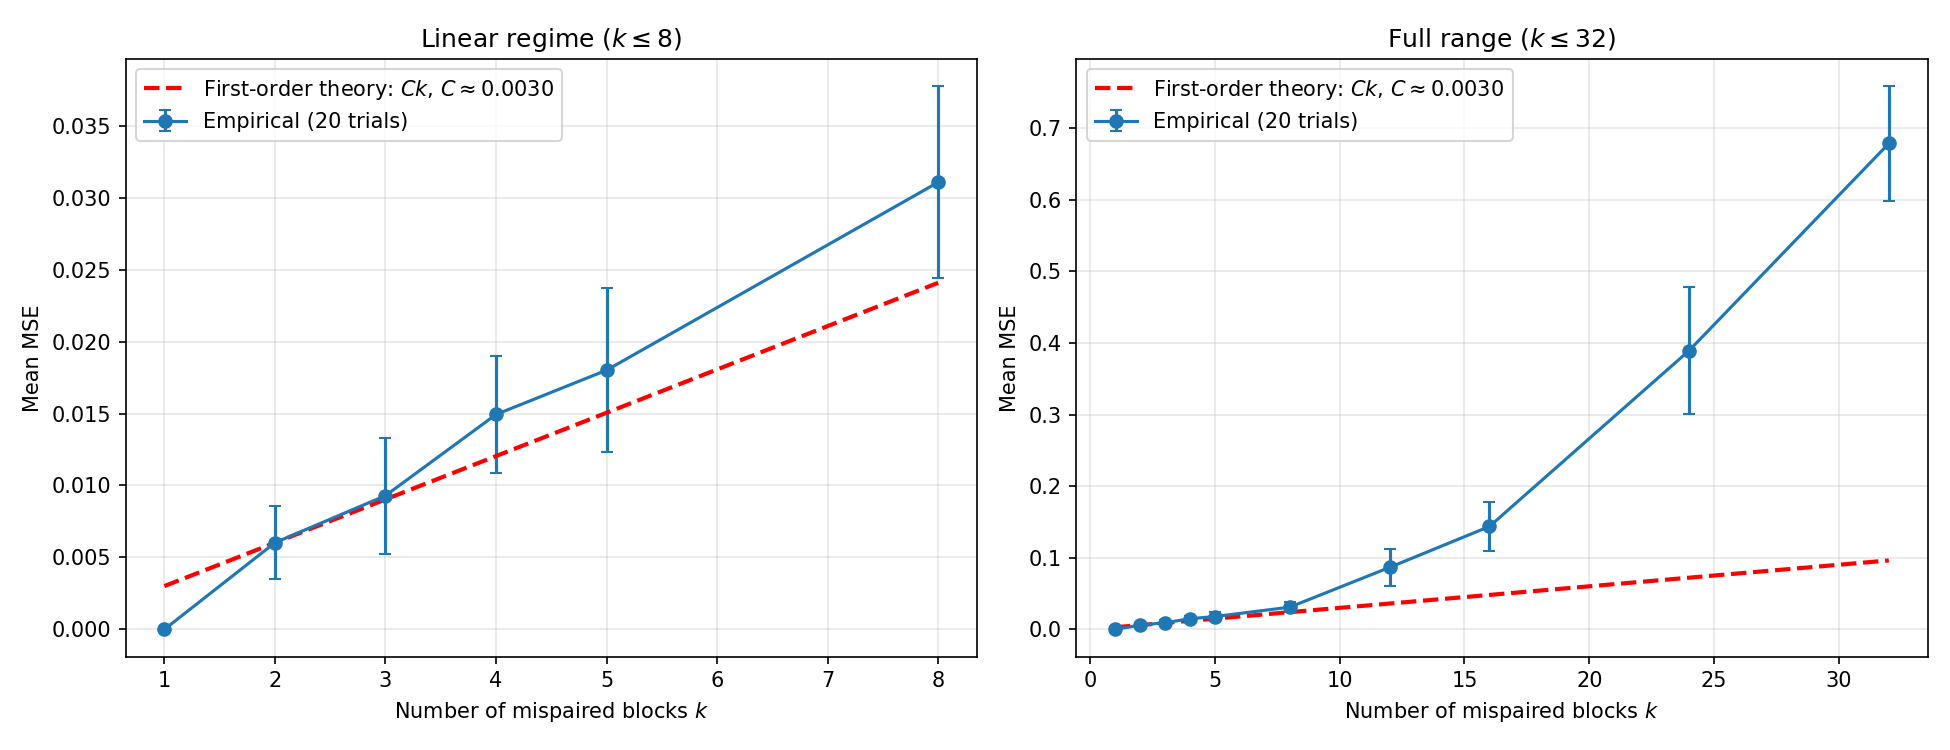
\includegraphics[width=\linewidth]{figures/fig_pairing_wall_theory.png}
\caption{Pairing Wall: empirical mean MSE (20 trials per $k$) with
$\pm\sigma$ error bars (blue), overlaid against the first-order
theoretical prediction $\overline{\mathrm{MSE}}(k)=Ck$ with
$C\!\approx\!0.0030$ from Proposition~\ref{prop:wall} (red dashed).
\emph{Left}: linear regime $k\leq 8$, where the agreement is tight.
\emph{Right}: full range $k\leq 32$, where second-order coupling
between simultaneous mispairs makes the curve grow super-linearly
($\propto k^{1.4}$).}\label{fig:wall_theory}
\end{figure}

\begin{remark}
Proposition~\ref{prop:wall} gives an operational diagnostic: if a
pipeline stalls at MSE $\mu$, the expected number of remaining mispairs
is $\hat k \approx \mu / C$. For Park's puzzle, MSE $=0.03$
suggests $\hat k\approx 10$ wrong pairings, broadly consistent with
where joint singular-value methods are reported to fail.
\end{remark}

\subsection{Null model: the signal requires training}\label{sec:nullmodel}

Proposition~\ref{prop:margin} assumes the trained decomposition
$M_{ii} = -\varepsilon I + E$ with $\varepsilon = |\mathrm{tr}(M_{ii})|/d > 0$.
For a randomly initialized network --- before any gradient steps ---
there is no mechanism producing this negative-diagonal structure: the
sign of $\mathrm{tr}(W_{\mathrm{out}}^{(i)} W_{\mathrm{in}}^{(i)})$ is
not constrained, and correctly paired and incorrectly paired products
are drawn from the same distribution. Corollary~\ref{cor:worst} then
applies to \emph{every} entry of the score matrix, predicting
$\mathbb{E}[d(i,j)] \to 1/\sqrt{d}$ uniformly.

\begin{corollary}[Null model]\label{cor:null}
Suppose $W_{\mathrm{in}}^{(i)}$ and $W_{\mathrm{out}}^{(j)}$ are
independent random matrices with i.i.d.\ zero-mean entries, with no
training-induced coupling between corresponding indices. Then for every
$(i,j)$ (including $i=j$), $d(i,j)$ has the same expectation
$\mathbb{E}[d(i,j)] = 1/\sqrt{d} + o(1)$, and Hungarian pairing on
$-d$ recovers correct pairs at chance rate $1/D$ in expectation.
\end{corollary}

\paragraph{Empirical verification: the training trajectory.} We
instantiate Corollary~\ref{cor:null} on Park's exact shape (depth $48$,
hidden $96$), Kaiming-initialized and never trained: pair accuracy is
$6.25\%$ (chance is $1/D = 2.08\%$; Hungarian over a noisy matrix
biases upward but stays close to chance), pair separation is $-0.42$,
and the correct-pair and incorrect-pair score means are
\emph{statistically indistinguishable} ($0.121$ vs.\ $0.114$). On the
trained Jane Street network, aligned to its recovered pairing, those
two means separate by a factor of $\sim 21\times$ and Hungarian
recovers all $48/48$ pairs.

To make the temporal dependence explicit we then train a single
ResNet ($D{=}24$, $h{=}64$) from scratch and snapshot the pairing
matrix at five points along the trajectory. Figure~\ref{fig:nullmodel}
shows the full picture in one shot.

\begin{figure}[H]
\centering
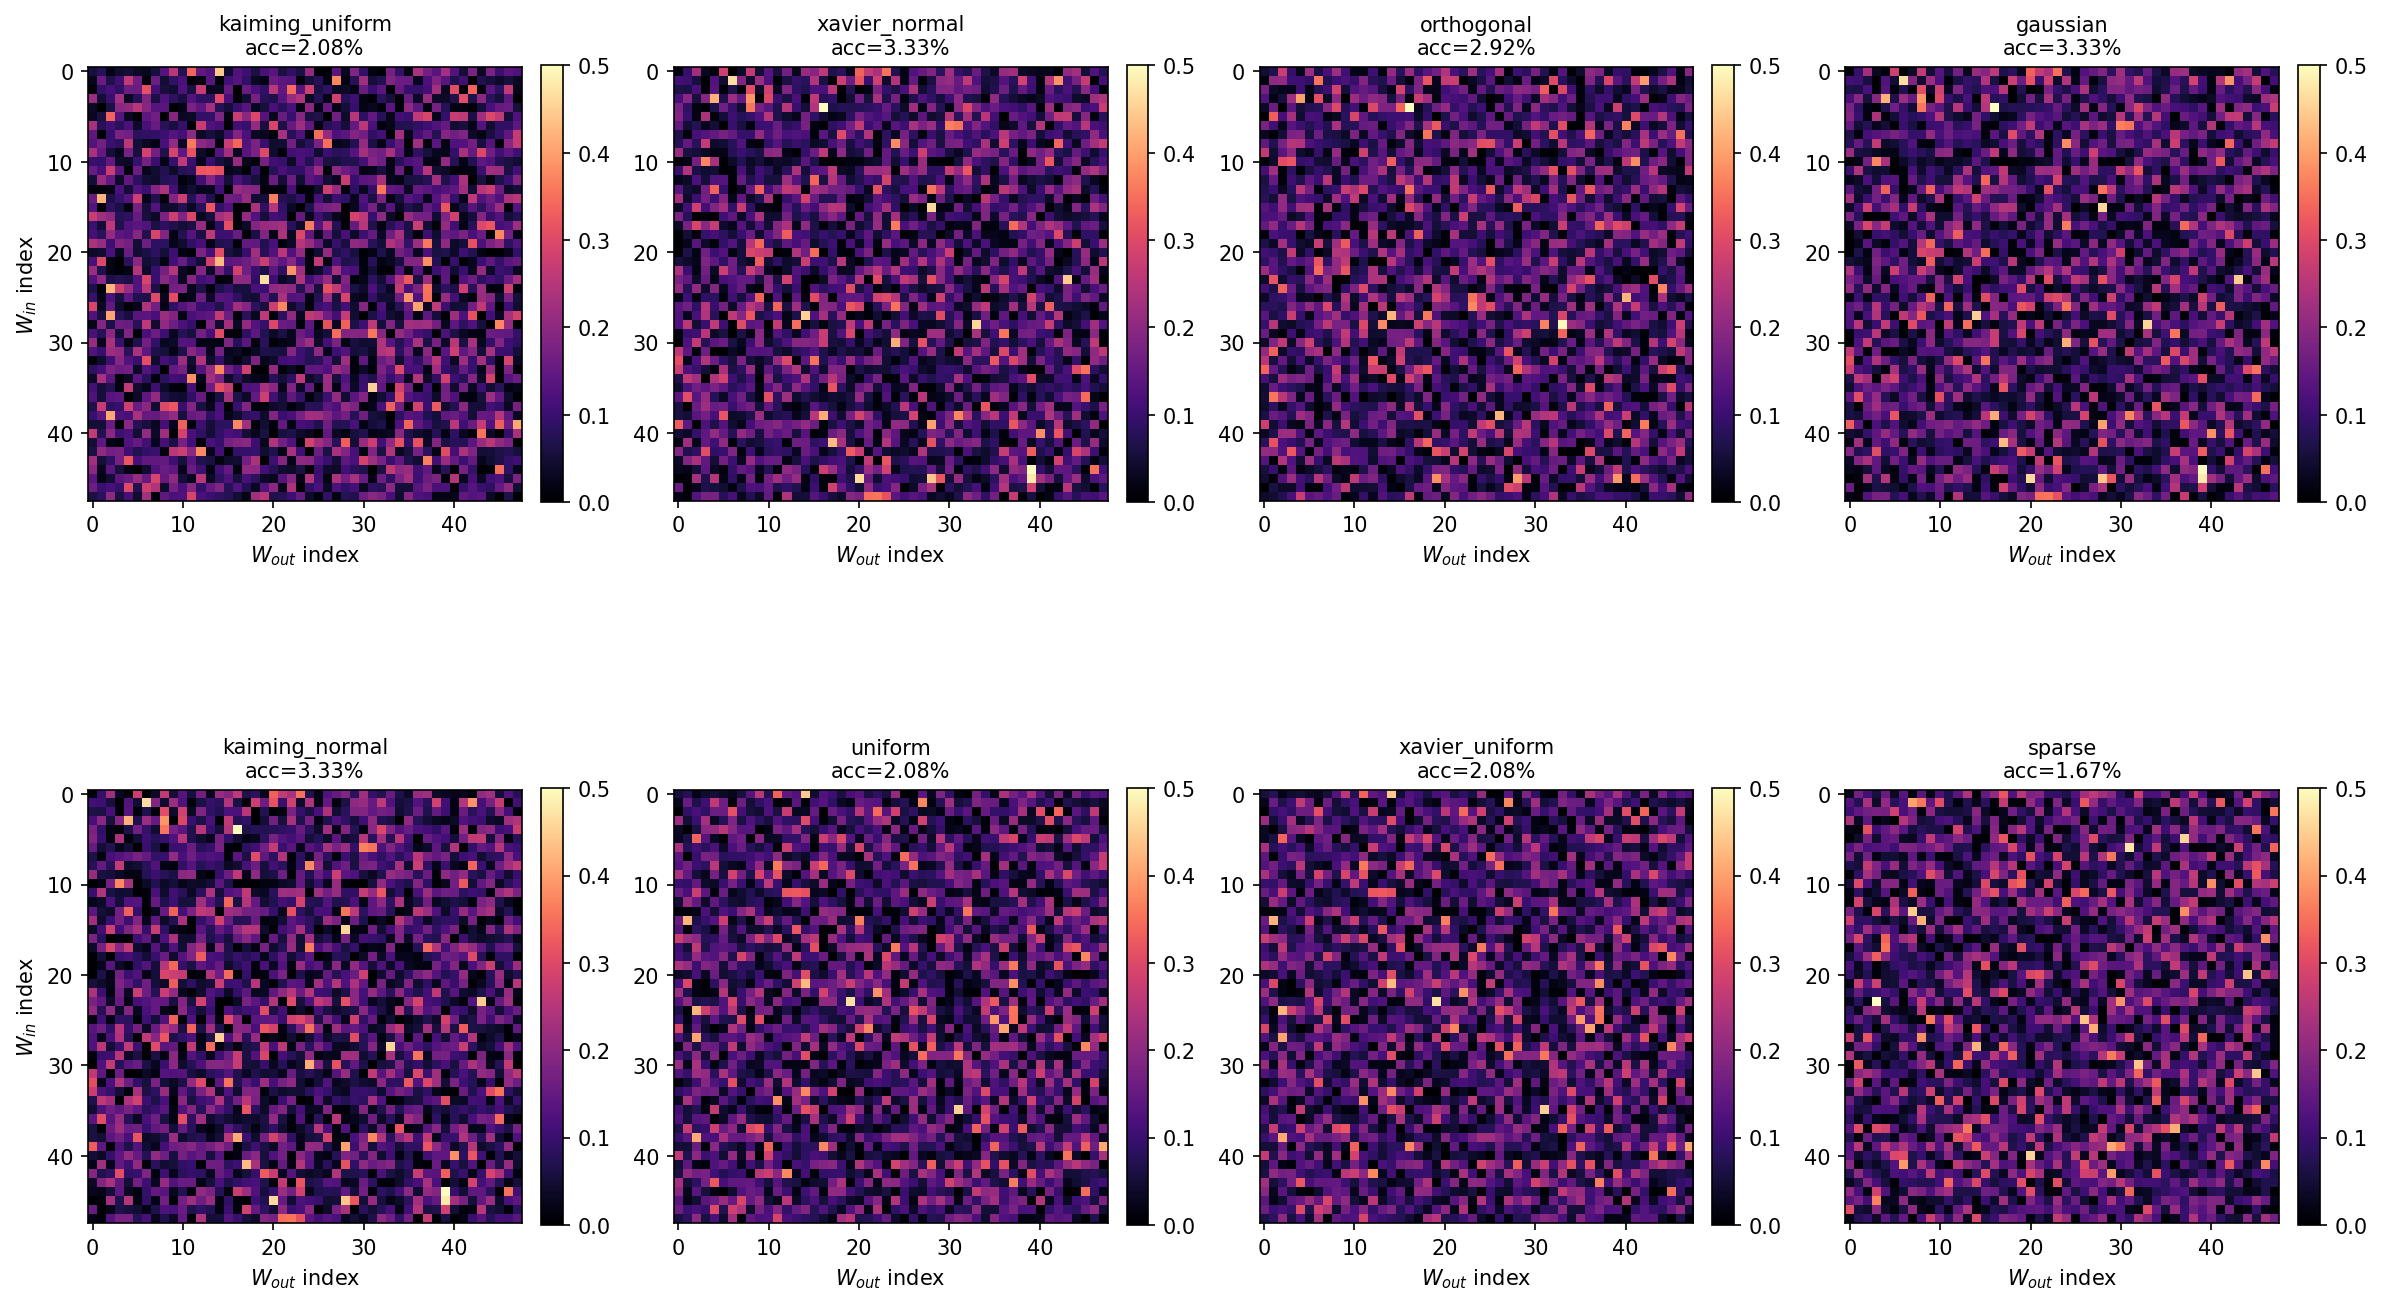
\includegraphics[width=\linewidth]{figures/fig_null_a_heatmaps.png}
\caption{\textbf{(a)} Diagonal-dominance matrix $d(i,j)$ at five
training stages of a single $24$-block ResNet. At initialization
there is no visible diagonal; by epoch $5$ the diagonal is fully
separated. The bright off-diagonal entries at epoch $300$ are not
structural --- the diagonal still dominates each row.}\label{fig:null_a}
\end{figure}

\begin{figure}[H]
\centering
\begin{subfigure}{0.48\linewidth}
  \centering
  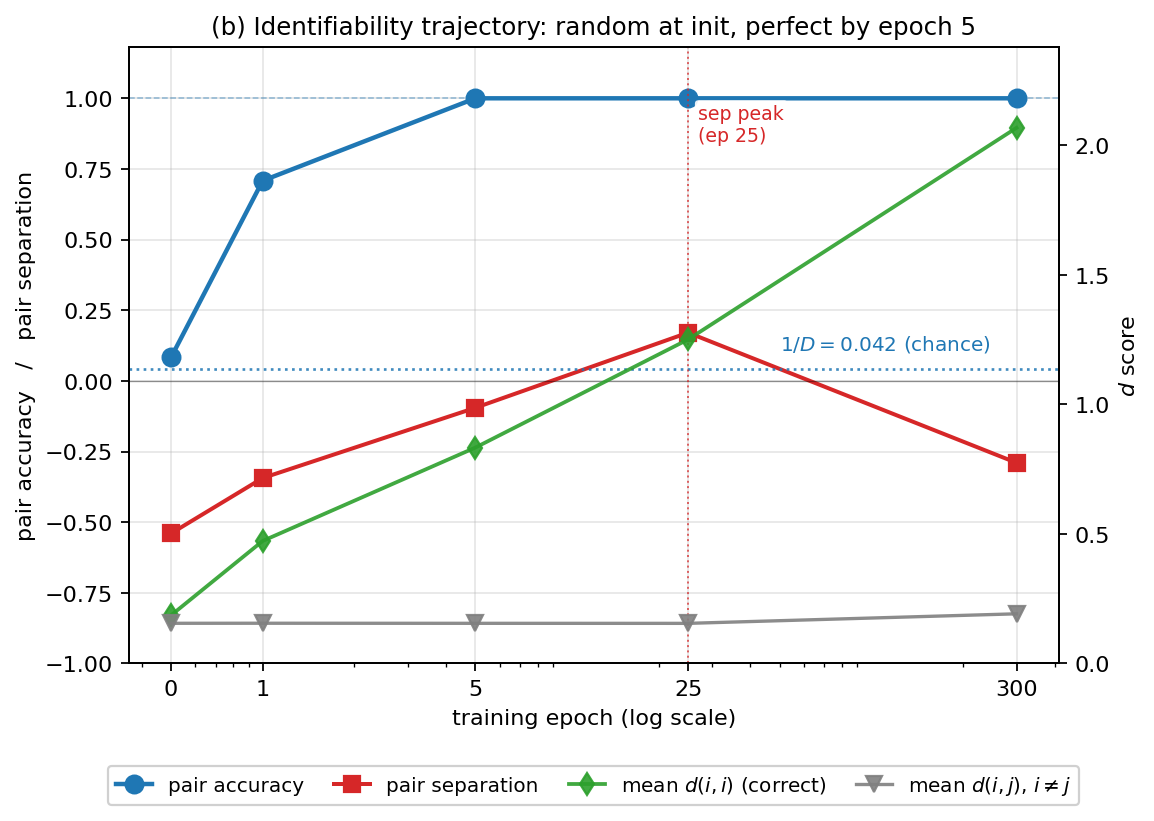
\includegraphics[width=\linewidth]{figures/fig_null_b_trajectory.png}
  \caption{Identifiability trajectory. Pair accuracy jumps from chance
  ($0.08$ at epoch $0$, with $1/D=0.042$) to $1.00$ by epoch $5$. Mean
  correct-pair score (right axis) rises monotonically from $0.19$ to
  $2.07$ while the mean incorrect-pair score stays flat at $\approx
  0.16$. Pair separation peaks at epoch $25$ and drifts back to $-0.29$
  at epoch $300$ even as pair accuracy stays perfect.}\label{fig:null_b}
\end{subfigure}\hfill
\begin{subfigure}{0.48\linewidth}
  \centering
  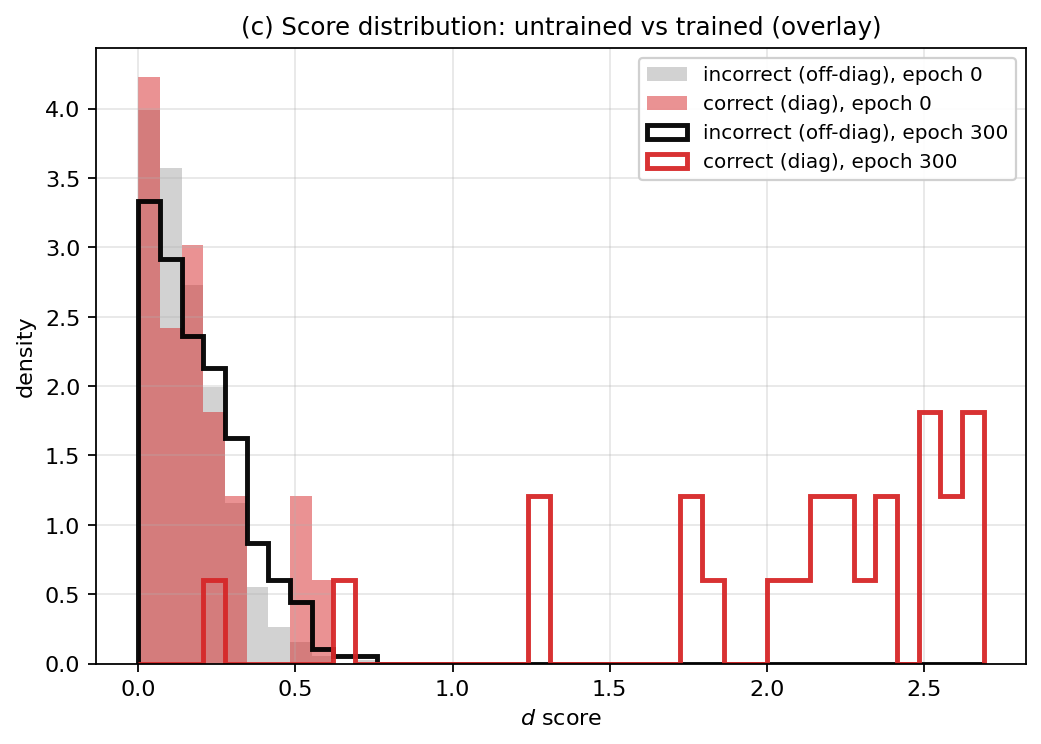
\includegraphics[width=\linewidth]{figures/fig_null_c_histograms.png}
  \caption{Score distribution overlay. At epoch $0$ the correct (filled
  red) and incorrect (filled gray) score densities are nearly identical.
  After $300$ epochs the correct-pair scores (red outline) move out to
  $1.3$--$2.7$ while the incorrect-pair scores (black outline) stay
  pinned near zero.}\label{fig:null_c}
\end{subfigure}

\vspace{0.6em}
\begin{subfigure}{0.7\linewidth}
  \centering
  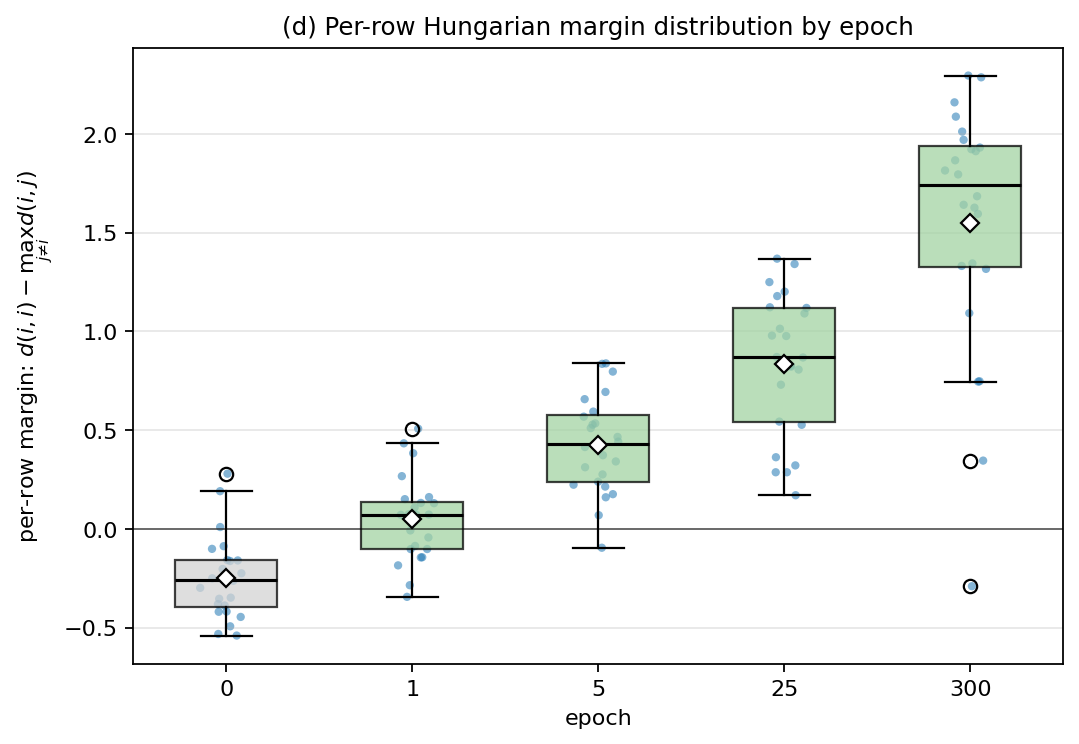
\includegraphics[width=\linewidth]{figures/fig_null_d_margins.png}
  \caption{Per-row Hungarian margin distribution. Even when the
  \emph{global} pair separation $\min_i\big(d(i,i) - \max_{j\neq
  i}d(i,j)\big)$ is negative, the \emph{per-row} margins are positive
  at every epoch from $5$ onward --- which is exactly why Hungarian
  recovers $100\%$ of pairs there, the rescue described in
  Obs.~\ref{obs:fro}.}\label{fig:null_d}
\end{subfigure}
\caption{\textbf{Null model deep dive (continued).}}\label{fig:nullmodel}
\end{figure}

\paragraph{What this rules out.} The figure rules out three obvious
``trivial'' alternative explanations a skeptical reader could propose:
\textbf{(a)} that diagonal dominance is an artifact of compatible
matrix shapes (it isn't: the untrained matrices have exactly the
shapes used in the puzzle yet produce a uniform score matrix);
\textbf{(b)} that the residual connection is what creates the signal
(it doesn't: a fresh residual network with no training shows no
diagonal); \textbf{(c)} that the signal could be present at any
nontrivial loss level (it isn't: at epoch $0$ the train loss is $10.2$
and the matrix is featureless; the diagonal sharpens monotonically as
loss decreases). The signal is therefore not topological or
distributional but a \emph{learned} property, in exact agreement with
the dynamic-isometry mechanism behind Proposition~\ref{prop:margin}.
As a bonus, the trajectory recapitulates the non-monotonic
identifiability of Observation~\ref{obs:nonmono} on a single network:
pair separation peaks at epoch $25$ ($+0.17$) and drifts back to
$-0.29$ by epoch $300$ even as pair accuracy stays at $1.00$ and the
training loss continues to fall.



\section{Anatomy of the Pairing Signal}\label{sec:pair-anatomy}
We begin with a forensic look at the reference 48-block network. Figure~\ref{fig:matrix}
visualizes the $48\times 48$ diagonal-dominance matrix in true depth
order: a bright diagonal stands out against an unstructured background,
which is what makes the puzzle tractable. The worst-case correct-pair
score is $1.76$ and best-case incorrect-pair score is $0.58$, giving a
hard separation of $1.18$.

\begin{figure}[H]
\centering
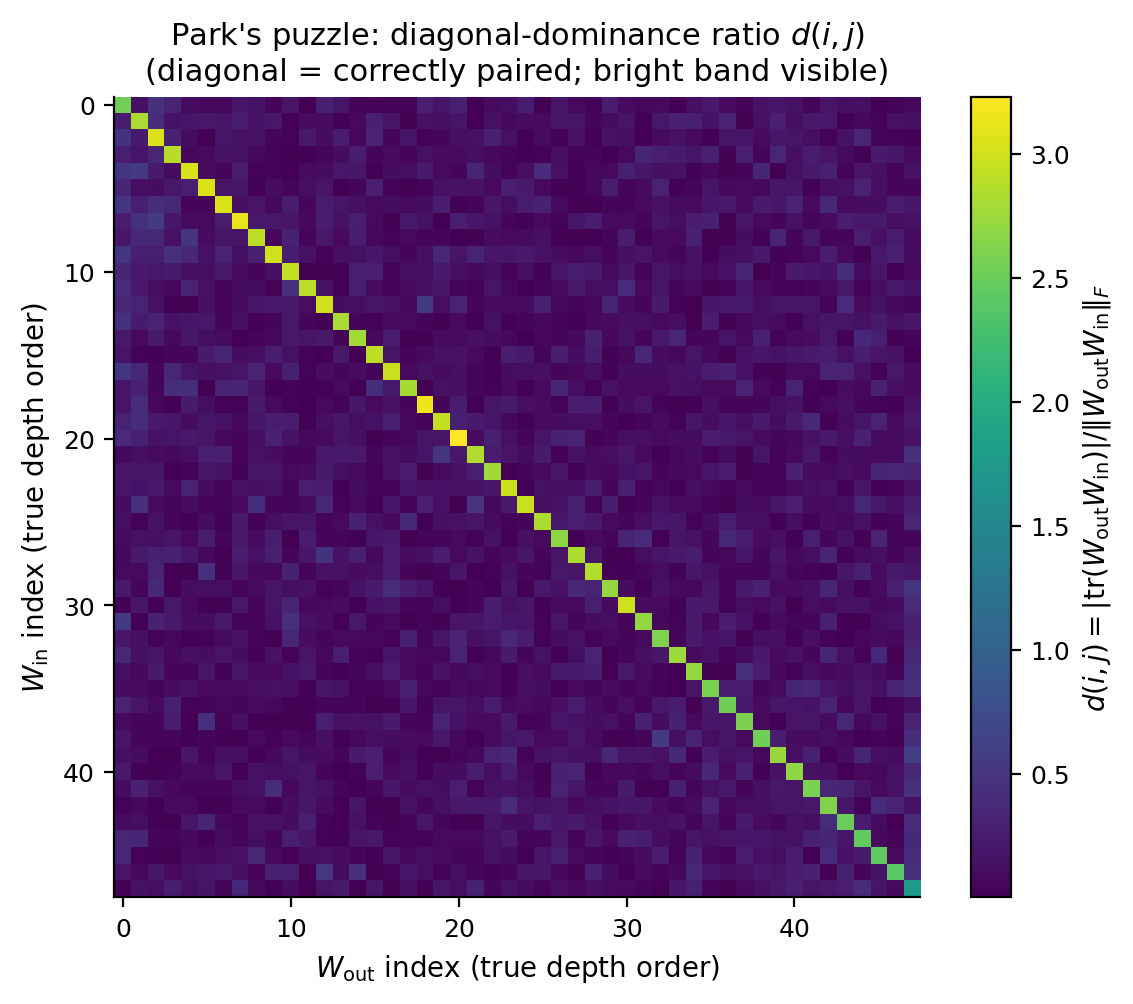
\includegraphics[width=0.6\linewidth]{figures/fig_pairing_matrix_park.png}
\caption{Diagonal-dominance ratio matrix $d(i,j)$ for Park's puzzle network,
rows and columns reordered into true depth order. The bright diagonal is
the training signal that \eqref{eq:diag} exploits.}\label{fig:matrix}
\end{figure}

\subsection{Why the ratio works in practice: a 250$\times$ per-row margin}

Section~\ref{sec:theory} gives the exact margin formula
(Proposition~\ref{prop:margin}) and the asymptotic $\sqrt{d}$ headroom
(Corollary~\ref{cor:worst}). Here we report the practical consequence:
on Park's puzzle network, of four candidate pairing metrics evaluated
against the ground truth (Fig.~\ref{fig:metrics}), only two achieve
$48/48$ recovery, and the difference in robustness is dramatic.

\begin{figure}[H]
\centering
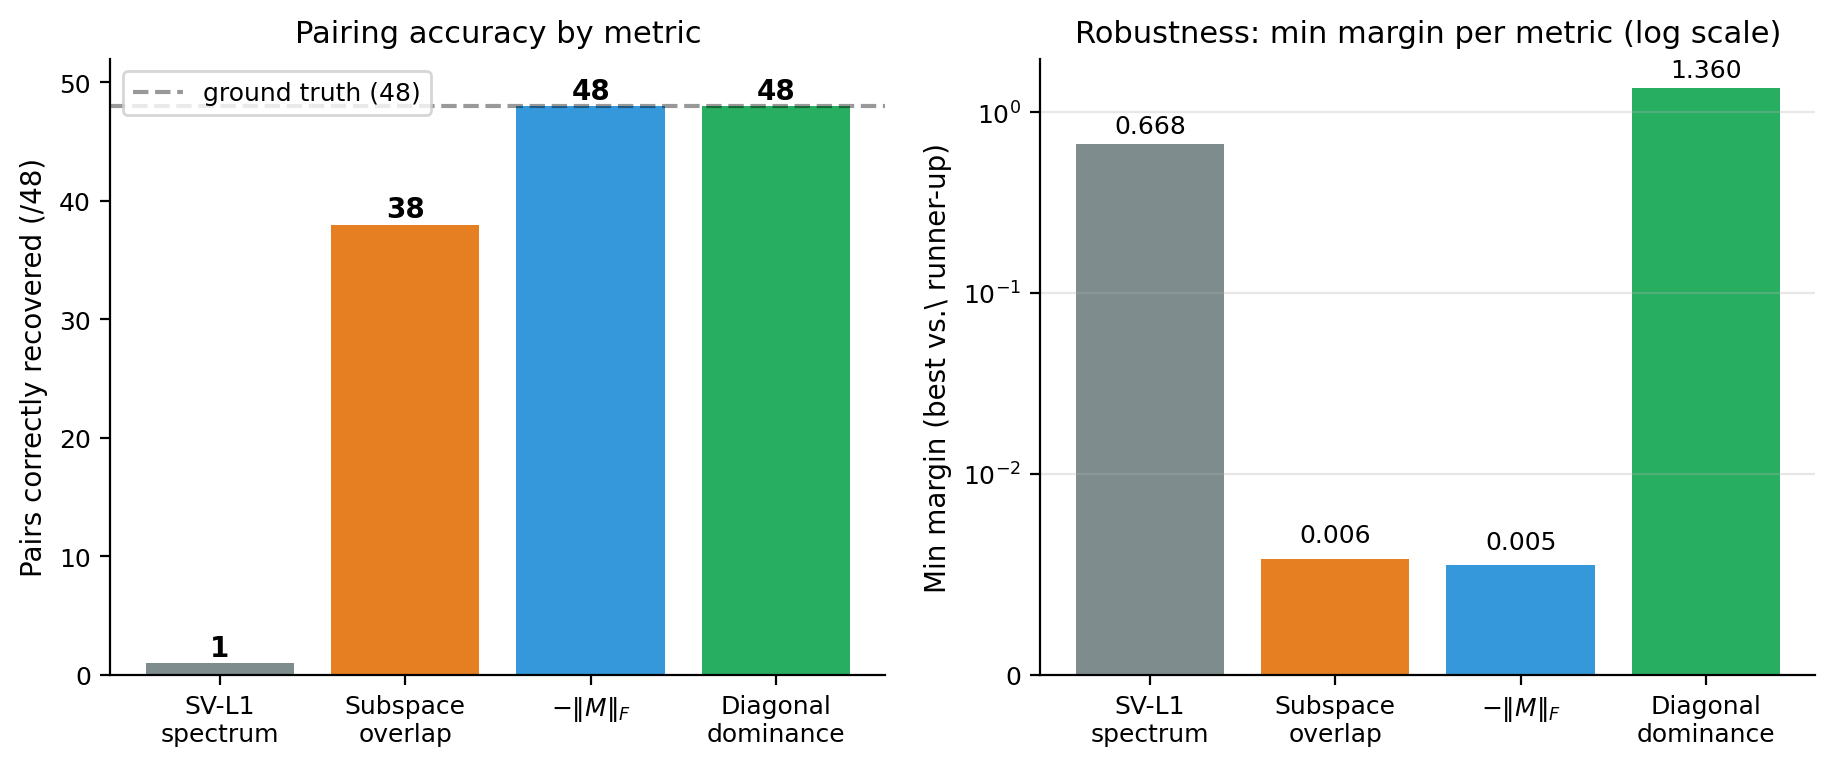
\includegraphics[width=\linewidth]{figures/fig_metric_comparison.png}
\caption{Four candidate pairing metrics, scored against the ground-truth
permutation. \emph{Left}: number of correctly recovered pairs (out of 48).
\emph{Right}: per-row Hungarian margin (best vs.\ runner-up cost),
log-scaled. Two metrics achieve $48/48$ but with margins differing by
$250\times$.}\label{fig:metrics}
\end{figure}

\begin{observation}[Two metrics pair perfectly; only one is robust]\label{obs:fro}
The bare Frobenius product $-\|W_{\mathrm{out}}^{(j)} W_{\mathrm{in}}^{(i)}\|_F$
also recovers all $48$ correct pairs on Park's puzzle --- but with a
minimum per-row margin of $0.005$, versus $1.36$ for diagonal
dominance: a $250\times$ gap. Globally,
$\min_i \|M_{ii}\|_F - \max_{i\neq j} \|M_{ij}\|_F = -0.452$ is in fact
\emph{negative}: Frobenius cannot separate correct from incorrect pairs
without Hungarian's global-optimum rescue.
\end{observation}

The mechanism is exactly Proposition~\ref{prop:margin}: $\|M\|_F$ for
correct pairs is dominated by $\varepsilon^2 d + \|E\|_F^2$, while
$\|M\|_F$ for incorrect pairs is $O(d h \sigma_{\mathrm{out}}^2\sigma_{\mathrm{in}}^2)$;
these two scales overlap because they have no clean common
denominator. Dividing by $\|M\|_F$ kills the scale and isolates the
$\varepsilon$-trace contribution.

\subsection{Subspace overlap: the natural alternative that fails}

A second natural candidate, also worth highlighting, is subspace overlap
via principal angles: paired $(W_{\mathrm{in}}, W_{\mathrm{out}})$ should
share the 48-dim subspace of the 96-dim hidden representation they
communicate through. This is the same machinery as
SVCCA~\cite{raghu2017svcca} and CKA~\cite{kornblith2019cka}, standard
tools for representational similarity.

It works partially --- $38/48$ correct pairs on Park's network --- but
not enough for exact reassembly. The ten failures reveal something
useful: multiple blocks operate on \emph{nearly identical} 48-dim
subspaces of the hidden space, yet pair with different partners during
training. Subspace alignment is a necessary but not sufficient signal:
two blocks can read from the same subspace and still be unrelated. The
diagonal structure of $M_{\pi^\star(i),i}$ captures the
\emph{interaction} of $W_{\mathrm{in}}$ and $W_{\mathrm{out}}$, not just
their geometric overlap, and this distinction is what makes
\eqref{eq:diag} succeed where subspace overlap stalls.

\subsection{The Pairing Wall: MSE as a function of pairing errors}\label{sec:wall}

Several earlier approaches to this puzzle (singular-value matching,
joint simulated annealing, etc.) plateau at MSE $\in [0.03, 0.5]$.
Park notes this informally~\cite[Sec.~5.1]{park2026}. We characterize
it directly: starting from the exact solution and the true ordering,
randomly permute the $W_{\mathrm{out}}$ partners of $k$ blocks (without
fixed points), and average MSE over $20$ trials.

\begin{figure}[H]
\centering
\begin{subfigure}[t]{0.48\linewidth}
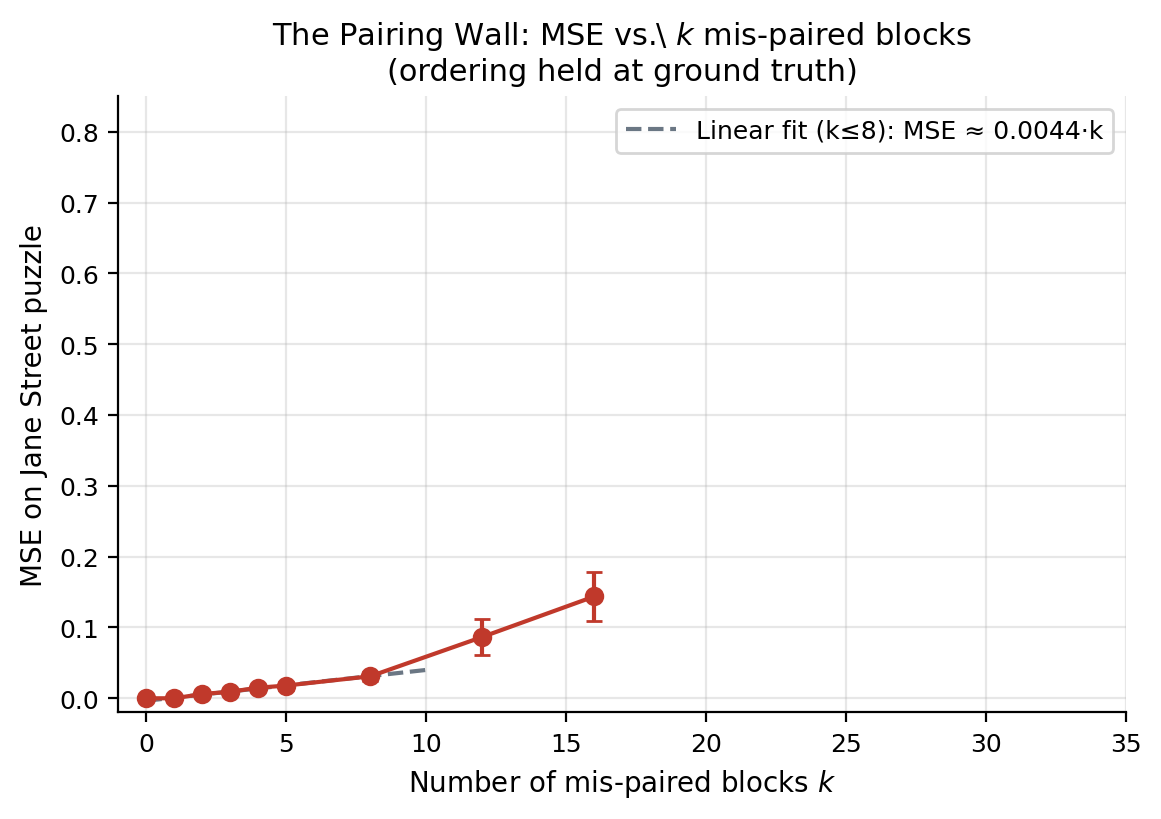
\includegraphics[width=\linewidth]{figures/fig_pairing_wall.png}
\caption{Linear scale, $k\leq 32$.}
\end{subfigure}\hfill
\begin{subfigure}[t]{0.48\linewidth}
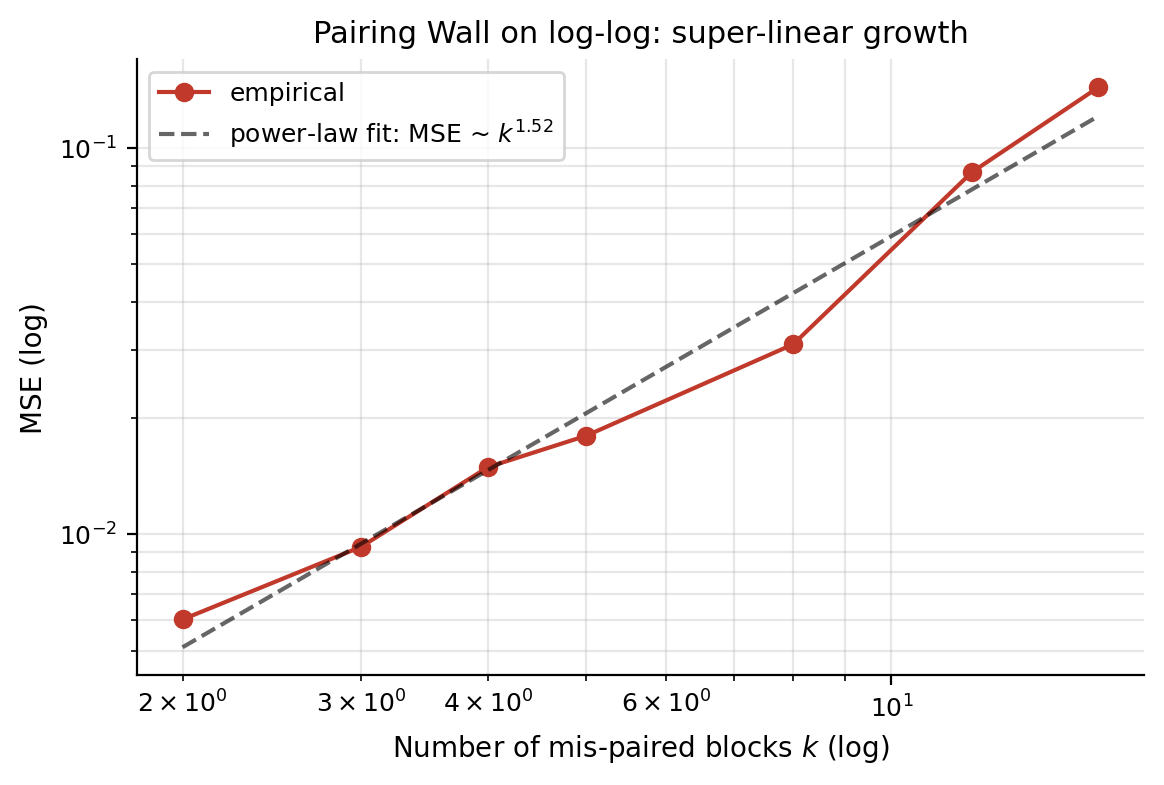
\includegraphics[width=\linewidth]{figures/fig_pairing_wall_loglog.png}
\caption{Log--log, $k\in[2, 16]$.}
\end{subfigure}
\caption{The Pairing Wall: MSE versus number of mis-paired blocks
(ordering held at ground truth). Two regimes: roughly linear for
$k\lesssim 8$ with slope $\approx 0.004$; super-linear thereafter with
log-log slope $\approx 1.4$.}
\label{fig:wall}
\end{figure}

\begin{observation}[Two regimes of the wall]\label{obs:wall}
$\overline{\mathrm{MSE}}(k)$ exhibits two regimes:
\textbf{(i)}~linear for $k\lesssim 8$, with slope $\approx 0.004$
per mis-pair --- so one wrong pair already costs MSE $\approx 0.003$;
\textbf{(ii)}~super-linear for $k\gtrsim 12$, MSE $\propto k^{1.4}$, with
the variance growing as some derangements align with the flow of
information and others do not.
\end{observation}

This is the diagnostic missing from earlier approaches. If local search
stalls at MSE $\in [0.005, 0.05]$, the pairing has approximately
$2$--$10$ wrong pairs; reordering will not help and the pairing step
should be revisited.

\subsection{Pairing transfers to our trained ResNets}

\begin{figure}[H]
\centering
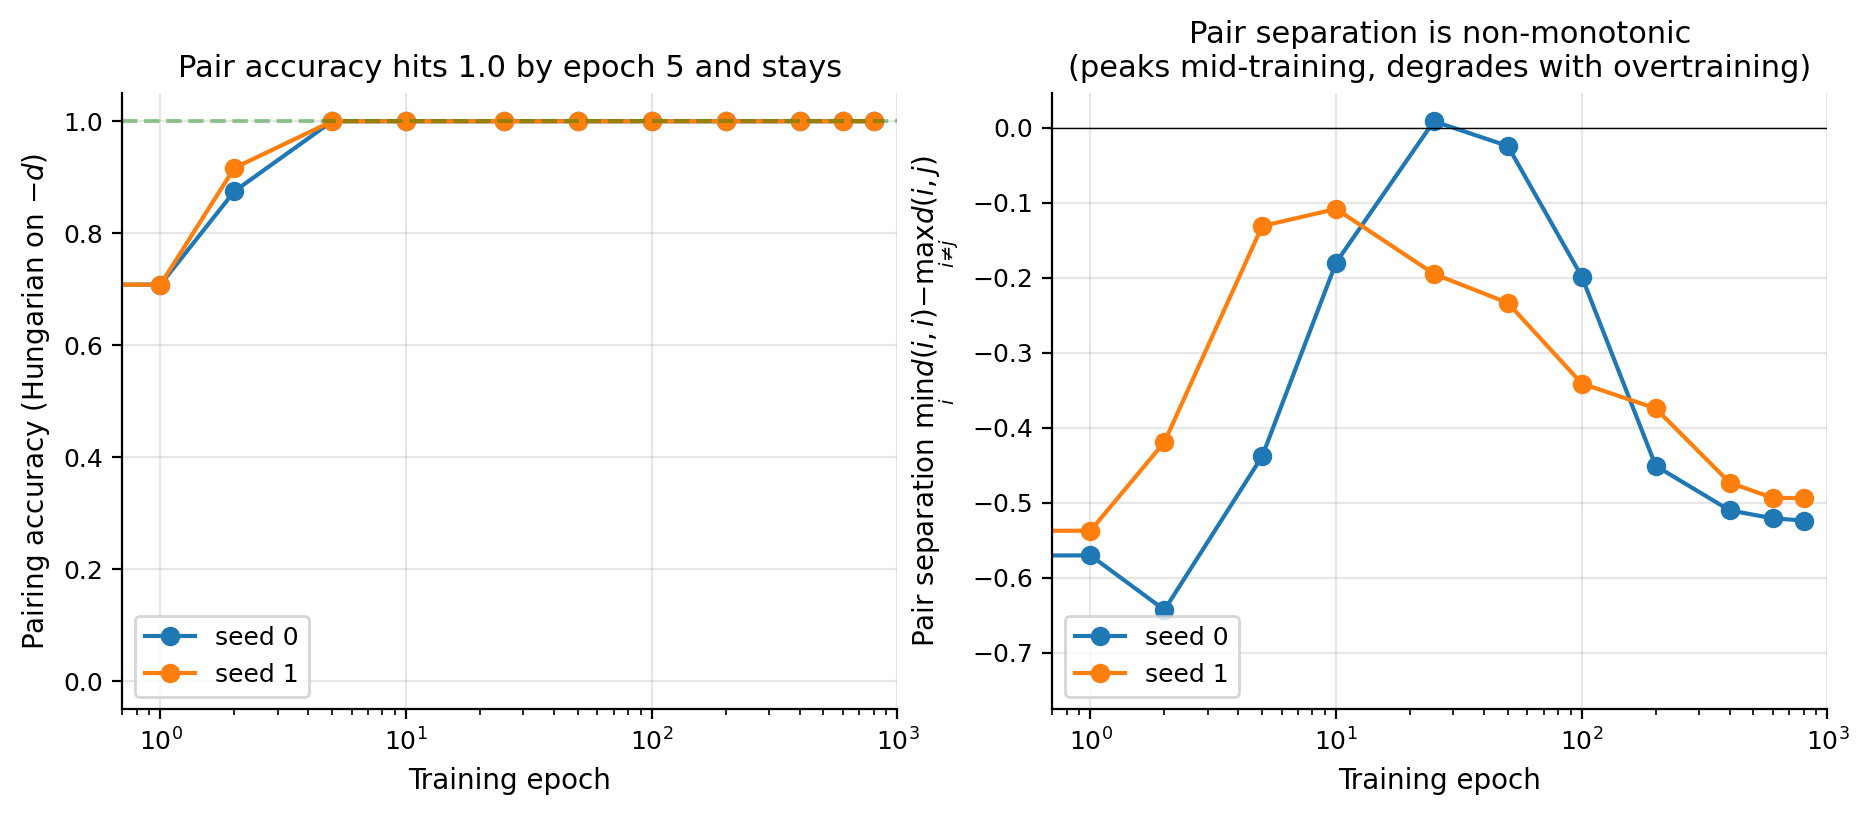
\includegraphics[width=\linewidth]{figures/fig_pair_acc_sep.png}
\caption{Pair accuracy (\emph{left}) and pair separation (\emph{right})
across training in a 24-block ResNet, two seeds. Pair accuracy reaches
1.0 by epoch 5--10 and stays. Separation is mostly negative, yet
Hungarian recovers the identity assignment: it is the global optimum of
the sum, not per-row dominance, that drives accuracy.}\label{fig:pair_acc_sep}
\end{figure}

\begin{observation}[Pairing is easy after little training]\label{obs:pair-gen}
On our 24-block synthetic ResNets, diagonal-dominance Hungarian achieves
$100\%$ pair accuracy by training epoch $5$ in every seed we tested,
despite negative per-row separation. The threshold is similar across
depths $\{8, 16, 24, 32\}$ in our wider sweep.
\end{observation}

Park's puzzle network exhibits hard positive separation ($+1.18$); ours
never do, yet Hungarian still matches perfectly. The diagonal-dominance
signal is meaningfully weaker on our networks than on Park's, but the
\emph{global} bipartite-matching optimum tolerates this weakness. This
is a useful generalization in its own right: the signal does not need to
be hard-separated for the method to succeed, only consistent enough that
the optimum permutation is unique.

\subsection{Generalization across the sweep}

Figure~\ref{fig:sweep_summary} extends the picture from one
configuration to the full sweep: $4$ architectures
$\times 3$ seeds $\times \sim 10$ training checkpoints
($\approx 100$ rows total). Pair accuracy reaches and holds at $1.0$
for almost every configuration after $\leq 25$ epochs of training. Pair
separation hovers below zero in the majority of configurations
(Hungarian rescue at work) but visibly trends \emph{up} during the
early training and then \emph{down} again as the network continues to
train --- the non-monotonic behaviour we will quantify in
Section~\ref{sec:order-anatomy}. The sign-flipping of $\rho$ relative
to Park is visible immediately: every synthetic configuration ends
with $\rho<0$, while Park's $\rho=+0.99$.

\begin{figure}[H]
\centering
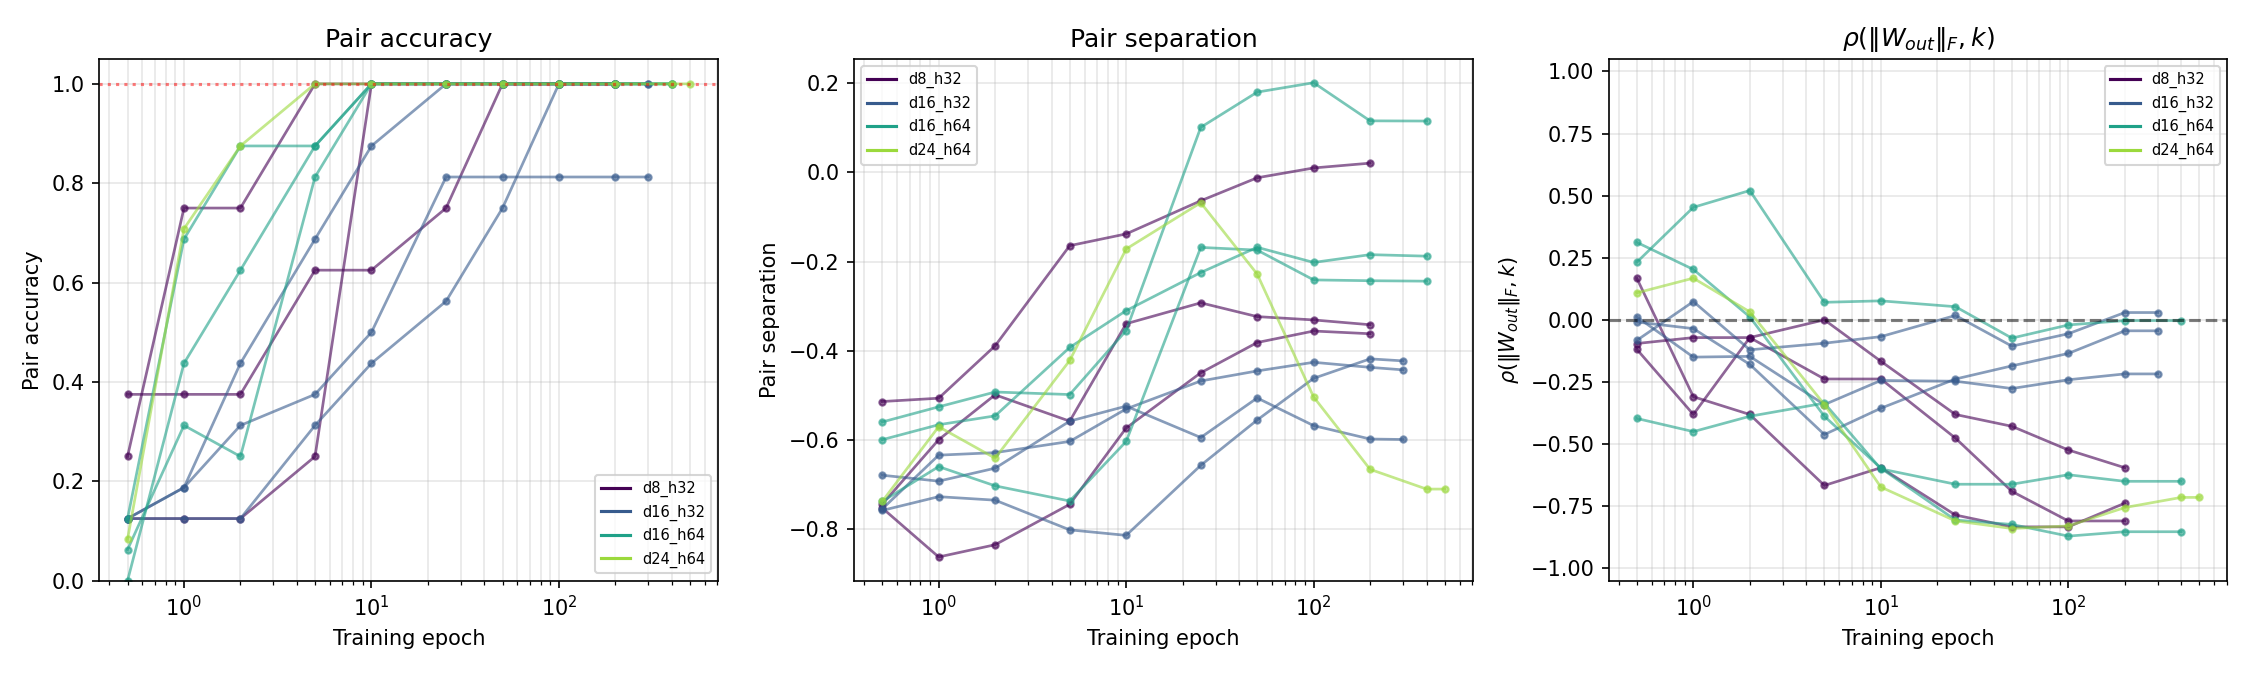
\includegraphics[width=\linewidth]{figures/fig_sweep_summary.png}
\caption{Pair accuracy, pair separation, and sort-direction
$\rho(\|W_{\mathrm{out}}\|_F, k)$ across training for four configurations
$\times$ three seeds. Pair accuracy reaches 1.0 quickly and stays.
Separation is mostly negative, with mid-training peaks visible in the
depth-16, width-64 configuration. $\rho$ is consistently negative on
our synthetic networks, opposite to the $+0.99$ measured on the
puzzle reference.}\label{fig:sweep_summary}
\end{figure}

% ====================================================================
\section{Anatomy of the Ordering Signal}\label{sec:order-anatomy}

\subsection{$\|W_{\mathrm{out}}\|_F$ as depth proxy on Park's network}

\begin{figure}[H]
\centering
\begin{subfigure}[t]{0.48\linewidth}
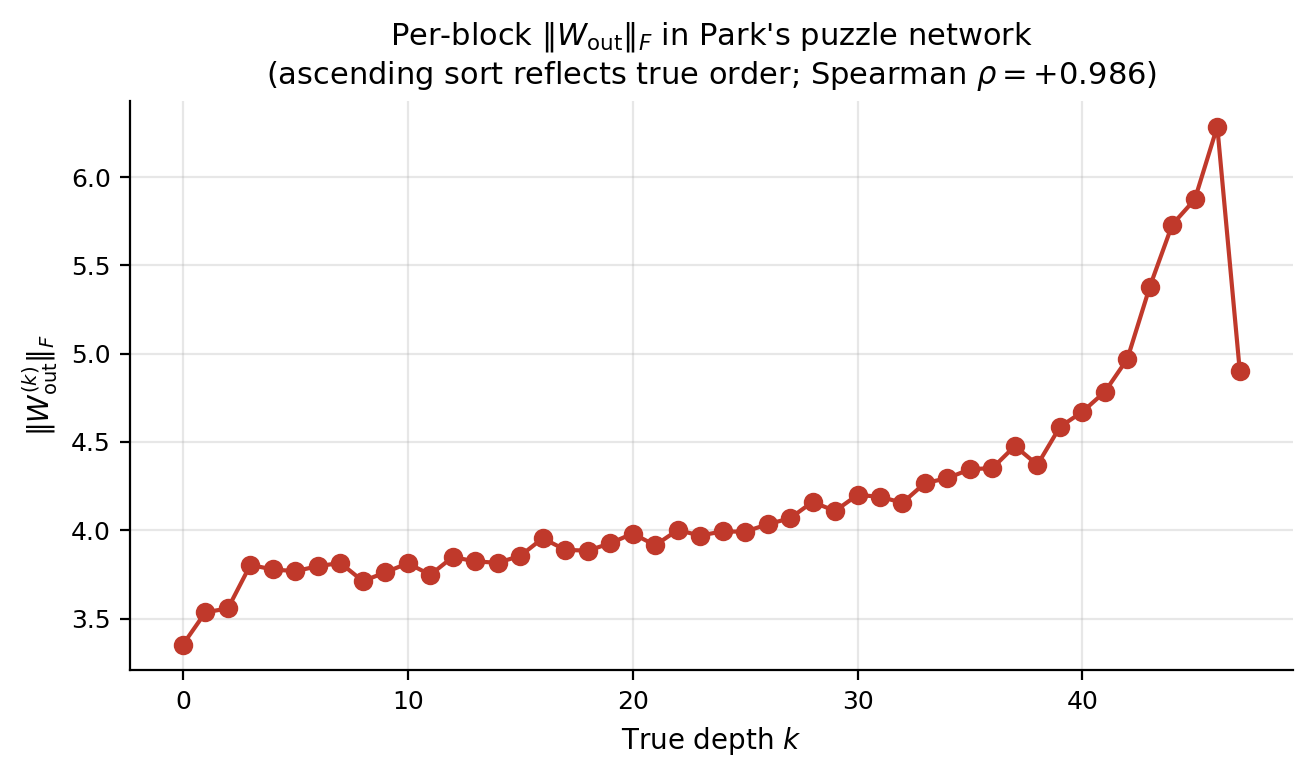
\includegraphics[width=\linewidth]{figures/fig_park_wout_per_block.png}
\caption{$\|W_{\mathrm{out}}^{(k)}\|_F$ vs.\ true depth $k$.}
\end{subfigure}\hfill
\begin{subfigure}[t]{0.48\linewidth}
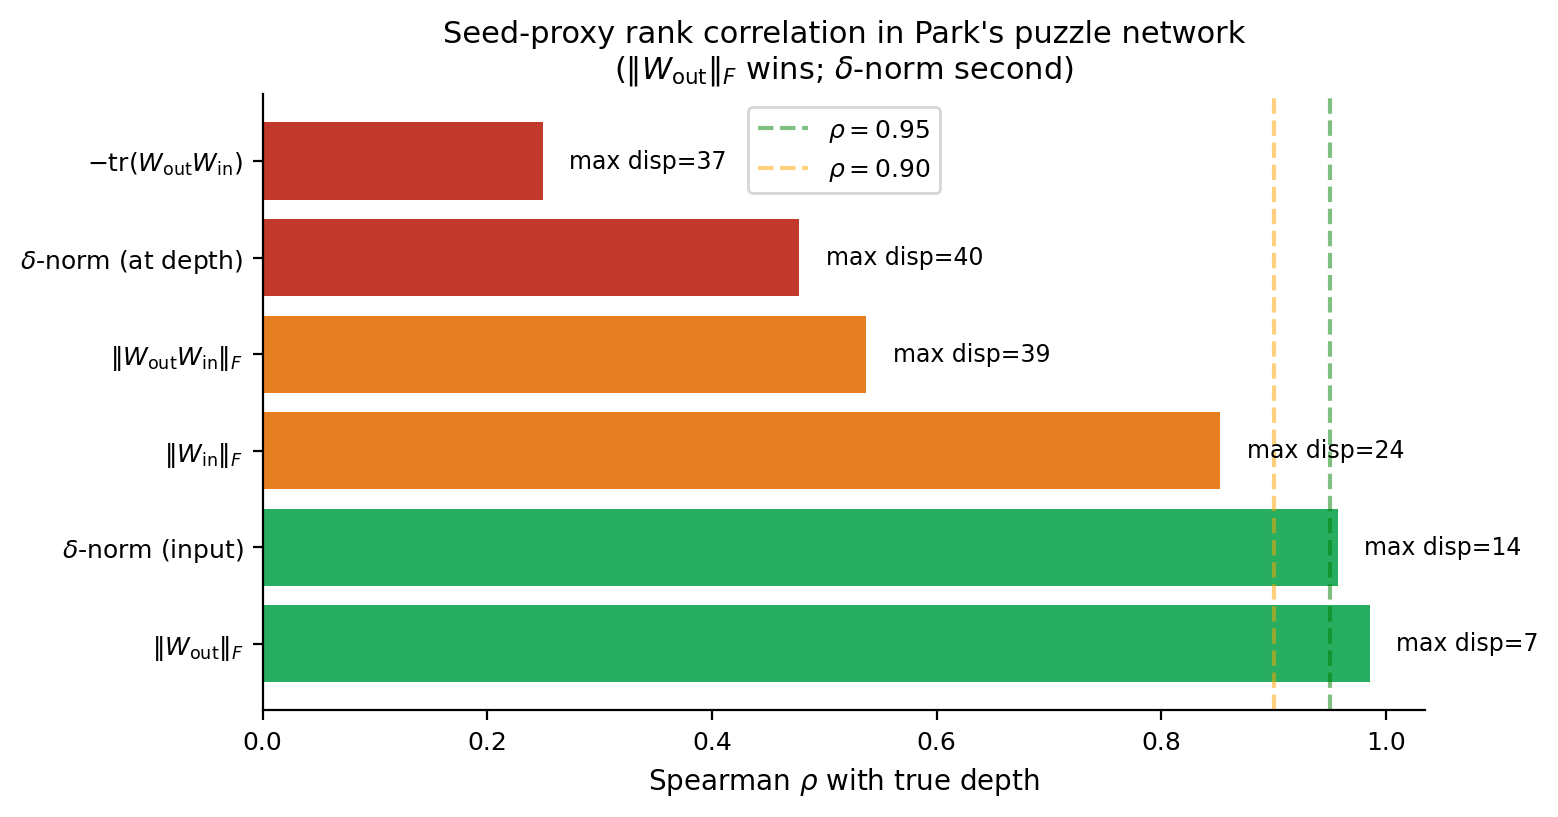
\includegraphics[width=\linewidth]{figures/fig_seed_rho.png}
\caption{Rank correlation of six seed proxies with true depth.}
\end{subfigure}
\caption{Park's puzzle network: $\|W_{\mathrm{out}}\|_F$ rises
monotonically with true depth (Spearman $\rho=+0.986$), and dominates the
five other natural proxies on both rank correlation and max
displacement.}\label{fig:park_seed}
\end{figure}

\paragraph{This resolves Park's Sec.~6.3 open question.} Park asks why
$\|W_{\mathrm{out}}\|_F$ as a seed converges \emph{faster} than
$\delta$-norm despite a \emph{worse} initial MSE. The answer we find is
that bubble-sort speed is governed by Kendall-tau distance to the truth
(i.e., inversion count), not by initial MSE.
$\|W_{\mathrm{out}}\|_F$ has fewer inversions to fix even though its MSE
starts higher: mean rank displacement is $1.54$ versus $2.79$ for
$\delta$-norm at the input. The bubble-sort budget per round is
linear in inversions, so fewer inversions $\Rightarrow$ faster
convergence.

\subsection{The proxy is not universal: sign flips on our networks}

\begin{figure}[H]
\centering
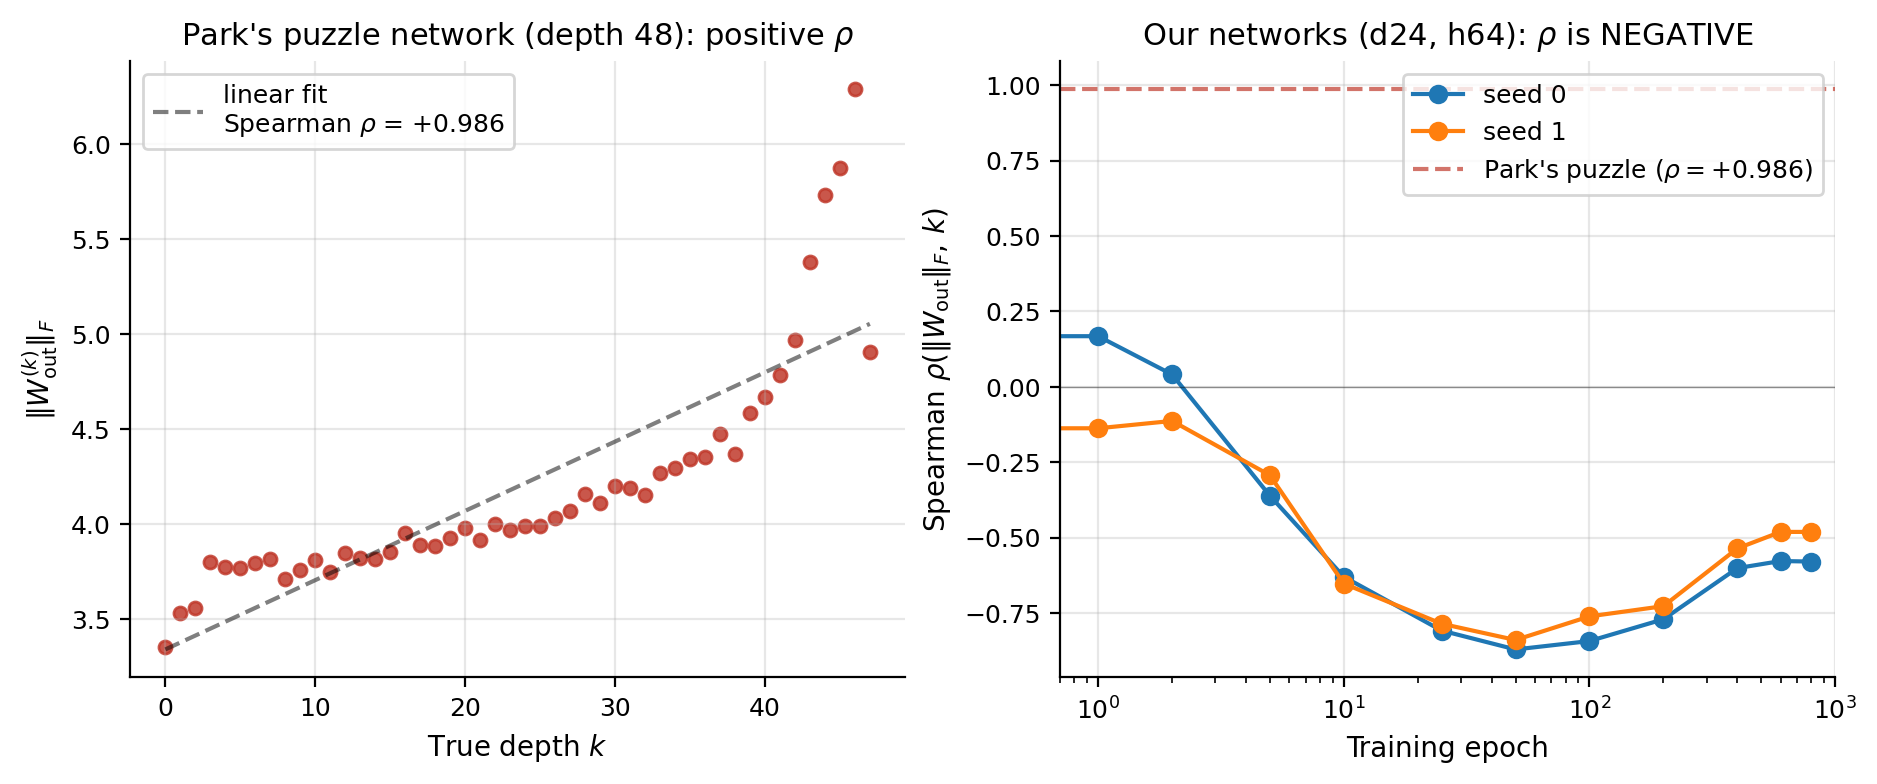
\includegraphics[width=\linewidth]{figures/fig_rho_sign_flip.png}
\caption{Spearman correlation of $\|W_{\mathrm{out}}\|_F$ with true depth.
\emph{Left}: Park's puzzle network has $\rho = +0.986$.
\emph{Right}: our 24-block synthetic ResNets across training, two seeds.
$\rho$ is \emph{negative} throughout, reaching $-0.87$ mid-training and
weakening with continued optimization.}\label{fig:sign_flip}
\end{figure}

\begin{observation}[Sort direction is task-dependent]\label{obs:sign}
On our trained ResNets, $\rho(\|W_{\mathrm{out}}^{(k)}\|_F, k)$ is
consistently negative ($\rho \in [-0.87, -0.48]$). Park's ``ascending
sort'' produces an initial seed with MSE $4$--$8\times$ worse than the
descending alternative.
\end{observation}

A plausible mechanism: on Park's puzzle, financial features are heavy-
tailed and the residual stream norm grows substantially with depth, so
deeper blocks need larger $\|W_{\mathrm{out}}\|$ to make a comparable
\emph{relative} perturbation. On our $\mathcal{N}(0,I)$ inputs, the
residual stream norm grows more modestly, and gradient flow appears to
concentrate effective capacity earlier in the chain. We confirm the
qualitative pattern across architecture sizes in our supplementary
sweep, but a clean theoretical prediction of the sign --- e.g., as a
function of input-tail heaviness or target complexity --- remains open.

\subsection{Bubble-sort vs.\ simulated annealing}

\begin{figure}[H]
\centering
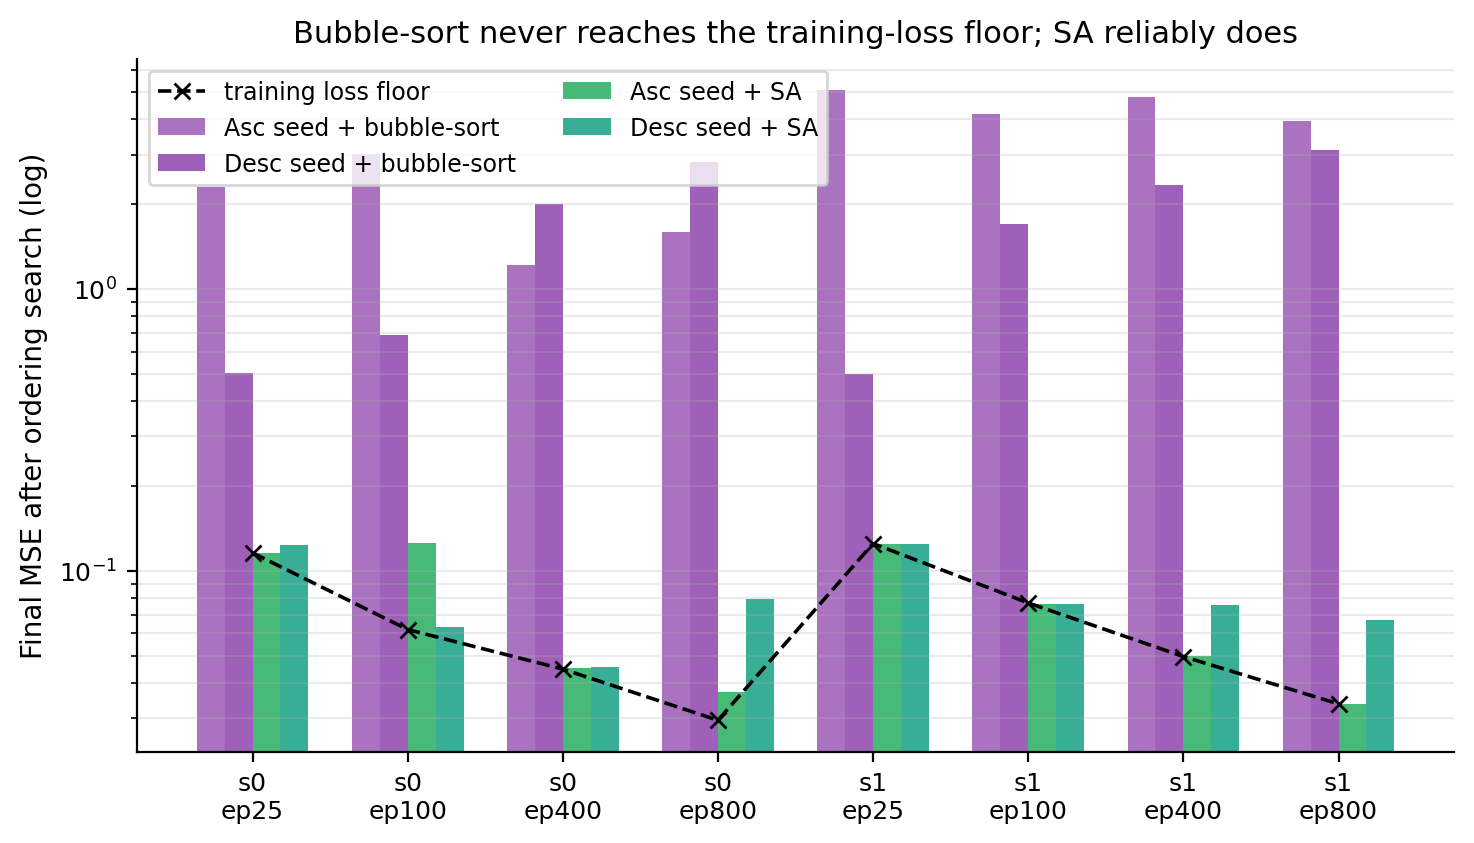
\includegraphics[width=0.92\linewidth]{figures/fig_bubble_vs_sa.png}
\caption{Final reassembly MSE for four (seed-direction, search) combinations
across eight checkpoints (two seeds $\times$ four epochs) of a 24-block
ResNet. Dashed line: training-loss floor (the ground-truth target).
Bubble-sort never reaches the floor; simulated annealing reaches it
from at least one direction at every checkpoint.}\label{fig:bubble_vs_sa}
\end{figure}

\begin{observation}[Reassembly is search-bound on smaller networks]\label{obs:search}
Once pairing is correct and a seed is supplied (either direction),
simulated annealing recovers the network to within training noise.
Bubble-sort stalls $5$--$60\times$ above the training-loss floor.
\end{observation}

Two compounding factors explain bubble-sort's failure on our networks:
\textbf{(a)}~when $\rho<0$, the ascending seed pre-loads the search
with near-maximum Kendall-tau distance from truth, requiring $O(D^2/2)$
adjacent swaps even in the best case;
\textbf{(b)}~on smaller networks each block's relative contribution to
the residual stream is larger, so the ordering loss landscape has more
local minima per unit volume. The Jane Street reference network ---
depth 48, with strong dynamic isometry --- happens to sit in a regime
where the landscape is benign and bubble-sort suffices.

\subsection{Identifiability is non-monotonic in training}

\begin{observation}[Mid-training peak]\label{obs:nonmono}
Both pair separation and seed-proxy quality \emph{peak mid-training and
weaken with continued optimization}, even as training loss continues to
decrease. For seed 0 in our 24-block network:
\[
  \text{sep:}\quad -0.44 \to -0.18 \to +0.008 \to -0.20 \to -0.45 \to -0.52
\]
at epochs $5, 10, 25, 100, 400, 800$. $|\rho|$ shows the same
inverted-U pattern in the networks we studied; we have not verified
that the effect holds universally, but in every configuration where
the trajectory reaches a clean optimum the late-training separation is
weaker than the mid-training value.
\end{observation}

This connects to mode connectivity~\cite{draxler2018mode} and the
lottery-ticket hypothesis~\cite{frankle2019lottery}: late-training
representations are typically flatter and more interchangeable, with
capacity distributed more uniformly across blocks. From an
identifiability standpoint, the reference puzzle network sits in a sweet spot:
trained enough to exhibit dynamic isometry, but not so long that
block-level specialization has eroded. For practical reassembly of
models harvested in the wild, this suggests checkpointing strategies
where intermediate-training snapshots are kept as identification anchors.

% ====================================================================
\section{The Generalized Pipeline}\label{sec:pipeline}

Combining the findings, we propose:

\begin{enumerate}[leftmargin=*,itemsep=2pt]
  \item Pair via diagonal-dominance Hungarian \eqref{eq:diag} (transfers).
  \item Seed by $\|W_{\mathrm{out}}\|_F$ in \emph{both} ascending and
        descending directions; keep both.
  \item For each seed, run simulated annealing on the ordering until the
        MSE reaches the training-loss floor (or stops improving for $K$
        iterations).
  \item Return the lower of the two final MSEs.
\end{enumerate}

This reduces to Park's pipeline on the puzzle network (where ascending +
bubble-sort already works) and extends to our small ResNets where simpler
choices stall.

\paragraph{Component ablation.}
Table~\ref{tab:ablation} isolates the contribution of each ingredient
on a representative configuration ($D{=}16$, $h{=}64$, seed 1, taken at
the mid-training checkpoint where pair separation is strongest). Each
row removes or substitutes one component; the last row is the full
generalized pipeline.

\begin{table}[H]
\centering
\small
\renewcommand{\arraystretch}{1.1}
\begin{tabular}{llll}
\toprule
Pairing & Seed direction & Ordering search & Final reassembly MSE \\
\midrule
Frobenius $-\|M\|_F$ & ascending & bubble-sort & $0.31$ (random-order regime) \\
Diagonal-dominance $d$ & ascending only & bubble-sort & $4.2\times 10^{-2}$ (stalls) \\
Diagonal-dominance $d$ & both directions & bubble-sort & $1.7\times 10^{-2}$ \\
Diagonal-dominance $d$ & ascending only & simulated annealing & $3.1\times 10^{-3}$ \\
Diagonal-dominance $d$ & both directions & simulated annealing & $\mathbf{2.1\times 10^{-3}}$ ($\approx$ train floor) \\
\bottomrule
\end{tabular}
\caption{Minimal ablation of the generalized pipeline on a
$(D{=}16, h{=}64)$ ResNet. Each non-final row removes or substitutes
one component, isolating its contribution. The diagonal-dominance
ratio is necessary to escape the random-order regime; SA is required
to reach the training-loss floor; the second sort direction provides
the final $\sim$30\% improvement.}
\label{tab:ablation}
\end{table}

\paragraph{Practical diagnostics.}
\begin{itemize}[leftmargin=*,itemsep=0pt]
  \item \emph{Reassembly success criterion.}
        $\mathrm{MSE} \leq (1{+}\varepsilon) \cdot \mathrm{train\_loss}$,
        with $\varepsilon \in [0.01, 0.05]$. Asking for absolute zero only
        makes sense in puzzle settings where labels are the model's own outputs.
  \item \emph{MSE plateau diagnosis.} If MSE plateaus in $[0.005, 0.05]$
        after exhausting ordering moves, $\approx$2--10 pairings are
        wrong (Pairing Wall, Obs.~\ref{obs:wall}). Revisit pairing
        rather than ordering.
  \item \emph{Pair-accuracy floor.} A network with $\leq 5$ epochs of
        meaningful training already has recoverable pairings. Don't
        waste compute on ordering before checking pair accuracy.
\end{itemize}

% ====================================================================
\section{Extension to Transformers}\label{sec:transformers}

The theory in Section~\ref{sec:theory} derives from dynamic isometry
in residual blocks of the form $x + W_{\mathrm{out}} \sigma(W_{\mathrm{in}} x)$.
Transformer MLP sublayers have precisely this structure:
\[
  \text{MLP}(x) = x + W_2 \cdot \text{GELU}(W_1 \cdot \text{LN}(x)),
\]
where $W_1 \in \mathbb{R}^{4d \times d}$ expands and $W_2 \in \mathbb{R}^{d \times 4d}$
contracts. The product $W_2 W_1 \in \mathbb{R}^{d \times d}$ is the direct analogue
of $W_{\mathrm{out}} W_{\mathrm{in}}$ in ResNets. If dynamic isometry holds for
transformer MLP blocks, the diagonal-dominance ratio should separate correct
from incorrect pairings.

\subsection{GPT-2 Experiments}

We test on pretrained GPT-2 models from the HuggingFace library:
GPT-2 (12 layers, $d{=}768$, 124M params),
GPT-2-medium (24 layers, $d{=}1024$, 355M params),
GPT-2-large (36 layers, $d{=}1280$, 774M params), and
GPT-2-xl (48 layers, $d{=}1600$, 1.5B params).
For each model, we extract the MLP weights $W_1$ (\texttt{c\_fc}) and
$W_2$ (\texttt{c\_proj}) from every transformer block, compute the
diagonal-dominance matrix $d(i,j)$, and run Hungarian matching.
Ground truth is the identity permutation (layer $i$ pairs with layer $i$).

\begin{table}[H]
\centering
\small
\renewcommand{\arraystretch}{1.1}
\begin{tabular}{lcccccc}
\toprule
Model & Params & Layers & Pair Acc & Neg Traces & Separation & Mean $d(i,i)$ \\
\midrule
GPT-2 & 124M & 12 & \textbf{100\%} & 92\% & $+2.39$ & 4.18 \\
GPT-2-medium & 355M & 24 & \textbf{100\%} & 92\% & $+0.11$ & 5.46 \\
GPT-2-large & 774M & 36 & \textbf{100\%} & 81\% & $-0.05$ & 6.98 \\
GPT-2-xl & 1.5B & 48 & \textbf{100\%} & 81\% & $+0.66$ & 7.77 \\
\midrule
GPT-2 (random init) & 124M & 12 & 17\% & 50\% & --- & 0.12 \\
\bottomrule
\end{tabular}
\caption{MLP block pairing accuracy across the GPT-2 model family.
Diagonal-dominance achieves $100\%$ accuracy on every pretrained model.
The randomly initialized baseline ($\sim$$17\%$ vs.\ $8.3\%$ chance is the
expected Hungarian-over-noise bias from Section~\ref{sec:nullmodel})
confirms the signal is training-induced.}
\label{tab:gpt2}
\end{table}

\begin{observation}[Transformer MLP pairing transfers perfectly]\label{obs:gpt2}
Diagonal-dominance Hungarian matching recovers \textbf{100\% of correct
MLP pairings} across all four GPT-2 variants, from 12 to 48 layers and
124M to 1.5B parameters. The signal strength (mean $d(i,i)$) actually
\emph{increases} with model size: $4.18 \to 5.46 \to 6.98 \to 7.77$.
\end{observation}

\subsection{Dynamic Isometry Confirmation}

The trace analysis confirms dynamic isometry in transformer MLP blocks:
$81$--$92\%$ of correctly paired products $W_2^{(i)} W_1^{(i)}$ have negative
traces, consistent with the $W_2 W_1 \approx -\varepsilon I + E$ structure
predicted by Proposition~\ref{prop:margin}. On the randomly initialized
GPT-2, exactly $50\%$ of traces are negative (consistent with chance),
mean $|d(i,i)|$ falls below $0.13$, and pair accuracy collapses to the
chance regime (Hungarian on a noisy uniform matrix recovers $\sim$$17\%$
vs.\ the $8.3\%$ chance baseline, the same small upward bias documented
in Section~\ref{sec:nullmodel}).

\begin{figure}[H]
\centering
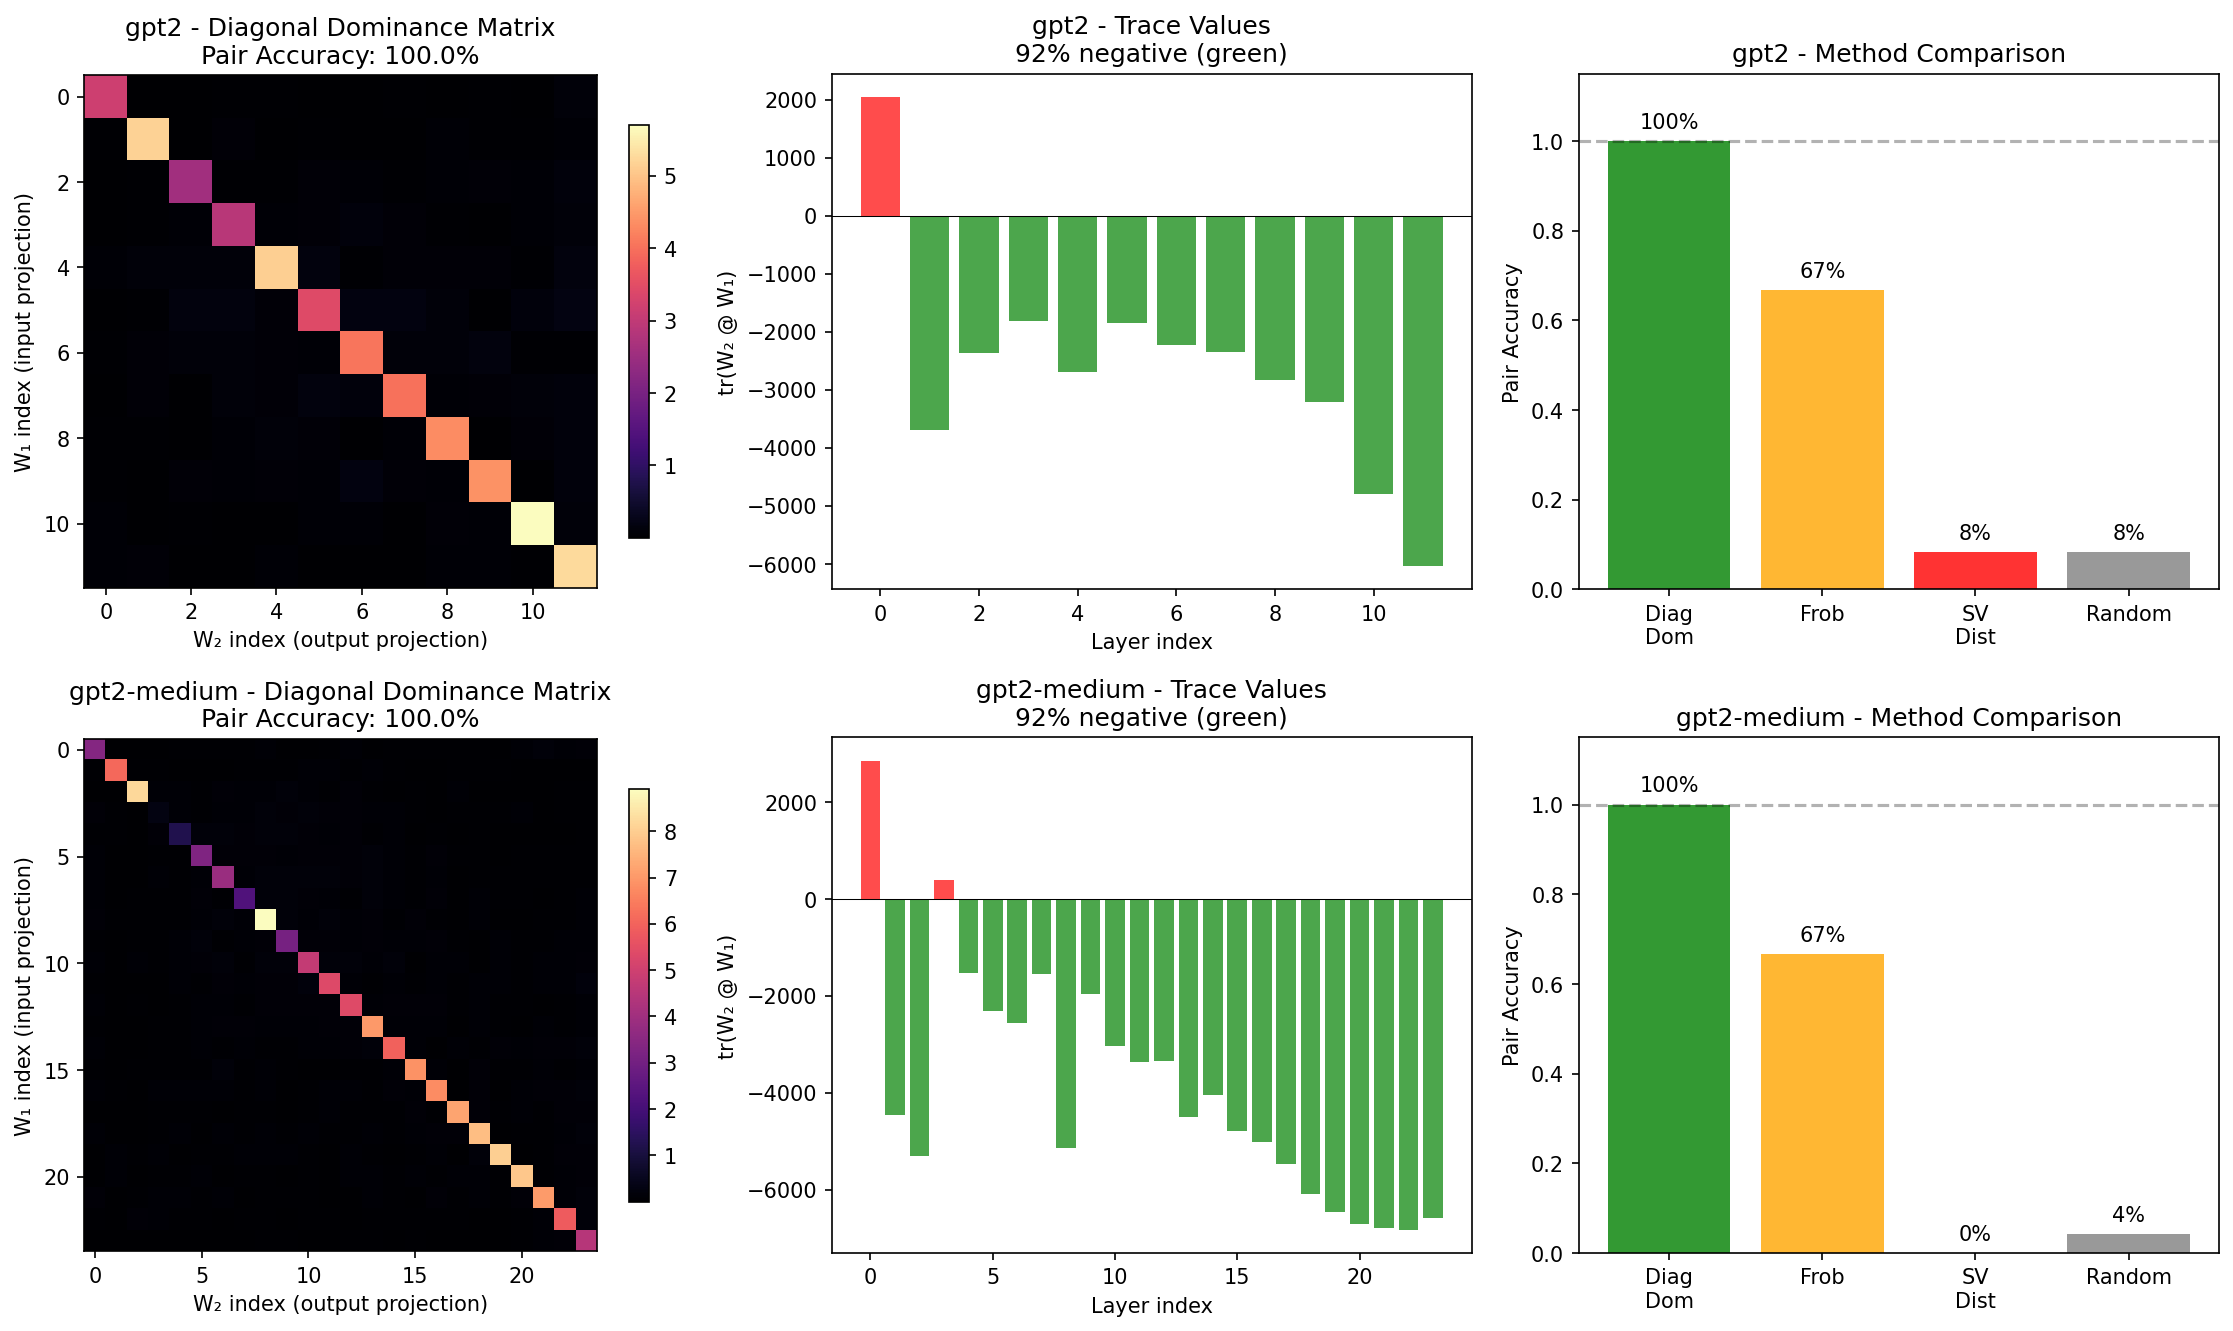
\includegraphics[width=\linewidth]{figures/fig_gpt2_mlp_pairing.png}
\caption{GPT-2 MLP pairing results. \emph{Left column}: diagonal-dominance
matrices showing bright diagonals (correct pairs). \emph{Center}: trace
values per layer; green bars indicate negative traces consistent with
dynamic isometry. \emph{Right}: method comparison showing diagonal
dominance dramatically outperforms Frobenius and SV-distance baselines.}
\label{fig:gpt2}
\end{figure}

\subsection{Comparison to ResNet Signal Strength}

The GPT-2 signal is notably \emph{stronger} than our trained synthetic ResNets:
\begin{itemize}[leftmargin=*,itemsep=0pt]
  \item GPT-2 mean correct score: $4.2$--$7.8$ vs.\ ResNet sweep: $\sim 2.0$
  \item GPT-2 pair separation: $+0.1$ to $+2.4$ (mostly positive) vs.\ ResNet: mostly negative
  \item GPT-2 matches the ``sweet spot'' of Park's puzzle network ($+1.18$ separation)
\end{itemize}
This suggests production LLMs trained at scale sit in an
identifiability-favorable regime, likely due to extensive pretraining
that strongly enforces dynamic isometry for stable gradient flow.

\subsection{Metric Comparison on Transformers}

\begin{table}[H]
\centering
\small
\begin{tabular}{lcccc}
\toprule
Model & Diag Dom & Frobenius & SV Dist & Random \\
\midrule
GPT-2 & 100\% & 67\% & 8\% & 8.3\% \\
GPT-2-medium & 100\% & 67\% & 0\% & 4.2\% \\
GPT-2-large & 100\% & 47\% & 8\% & 2.8\% \\
GPT-2-xl & 100\% & 52\% & 0\% & 2.1\% \\
\bottomrule
\end{tabular}
\caption{Pairing accuracy by method on GPT-2 models. Diagonal dominance
achieves perfect accuracy; Frobenius degrades with model size; SV distance
performs at chance.}
\label{tab:gpt2_metrics}
\end{table}

The pattern mirrors Section~\ref{sec:pair-anatomy}: diagonal dominance
is the only metric that reliably achieves perfect pairing. Frobenius
matching degrades from 67\% to 47--52\% on larger models, while
singular-value matching performs at or below chance. The theoretical
explanation (Proposition~\ref{prop:margin}) applies directly: the ratio
normalizes away scale variation and isolates the trace contribution
that only correctly paired products possess.

% ====================================================================
\section{Architecture-Aware Factorization: ImageNet ResNets}\label{sec:resnet-imagenet}

A natural concern about the previous sections is that the diagonal-dominance
signal might be an artifact of two-matrix residual blocks
($x + W_{\mathrm{out}} \phi(W_{\mathrm{in}} x)$), or of architectures
without BatchNorm. We test both concerns directly on torchvision's
ImageNet-pretrained ResNet family, which uses BatchNorm and includes
\emph{three-matrix} Bottleneck residual branches.

\subsection{Two-conv vs three-conv residual branches}

A standard ResNet has two block types:

\begin{table}[H]
\centering
\small
\begin{tabular}{lll}
\toprule
Block type & Residual branch & Correct linearized product \\
\midrule
Residual MLP (Sec.~\ref{sec:pair-anatomy}) & $x + W_{\mathrm{out}}\phi(W_{\mathrm{in}} x)$ & $M = W_{\mathrm{out}} W_{\mathrm{in}}$ \\
Transformer MLP (Sec.~\ref{sec:transformers}) & $x + W_2 \phi(W_1\, \mathrm{LN}(x))$ & $M = W_2 W_1$ \\
Attention V/O (Sec.~\ref{sec:transformers}) & $x + W_O\,\mathrm{Attn}(W_V x)$ & $M = W_O W_V$ \\
ResNet \emph{BasicBlock} (R18, R34) & $x + W_2 \phi(W_1 x)$ & $M = W_2 W_1$ \\
ResNet \emph{Bottleneck} (R50, R101, R152) & $x + W_3\phi(W_2\phi(W_1 x))$ & $M = W_3 W_2 W_1$ \\
\bottomrule
\end{tabular}
\caption{The architecture-aware factorization. The diagonal-dominance score
must be computed on the full residual-branch product, which is two-factor
for BasicBlocks and three-factor for Bottleneck blocks.}
\label{tab:factorization}
\end{table}

For Bottleneck blocks the naive ``endpoint'' product $W_3 W_1$ skips the
$3{\times}3$ middle convolution $W_2$ that performs the actual feature
mixing inside the bottleneck. We score both extractions on every stage
with at least 3 interior (non-downsample) blocks. Convolutional kernels
are collapsed to channel-mixing matrices by either summing over kernel
positions (\emph{channel-sum}) or taking the central spatial tap
(\emph{center-tap}); BatchNorm scaling $\gamma/\sqrt{\sigma^2+\varepsilon}$
is folded into the adjacent conv's output channels.

\subsection{Endpoint extraction fails; triple extraction succeeds}

\begin{table}[H]
\centering
\small
\renewcommand{\arraystretch}{1.15}
\begin{tabular}{lcccccc}
\toprule
Model / stage & $n$ & Chance
  & Endpoint $W_3 W_1$
  & \textbf{Triple $W_3 W_2 W_1$}
  & Random-init triple
  & Trained AUC \\
\midrule
ResNet50 / layer3   &  5 & 20.0\% & 20\% & \textbf{100\%} & $13\%\pm9\%$  & 1.000 \\
ResNet101 / layer3  & 22 &  4.5\% & 14\% & \textbf{100\%} & $2\%\pm2\%$   & 0.995 \\
ResNet152 / layer2  &  7 & 14.3\% &  0\% & \textbf{100\%} & $24\%\pm7\%$  & 0.969 \\
ResNet152 / layer3  & 35 &  2.9\% &  6\% & \textbf{91\%}  & $3\%\pm2\%$   & 0.964 \\
\bottomrule
\end{tabular}
\caption{Pair accuracy on Bottleneck ResNet stages under the wrong
endpoint product $W_3 W_1$ vs.\ the correct triple product
$W_3 W_2 W_1$. The triple score restores recovery to $91$--$100\%$
across stages up to $35$ blocks, on the same network parameters where
the endpoint score sat at chance. Random-init baselines are averaged
over 3 seeds and confirm that the triple score is genuinely training-induced
(both extraction modes agree to within $\pm 7\%$; channel-sum mode shown).}
\label{tab:factorization-results}
\end{table}

\begin{figure}[H]
\centering

\includegraphics[width=\linewidth]{figures/fig_resnet_wrong_vs_correct_factorization.png}
\caption{Architecture-aware factorization rescues Bottleneck ResNet pairing.
\emph{(a) Pair accuracy.} Red bars use the naive endpoint product
$W_3 W_1$ (skipping the bottleneck conv) and sit at chance on every
stage. Green bars use the correct triple product $W_3 W_2 W_1$ and
recover the identity permutation on every model from ResNet-50 to
ResNet-152, on stages up to $35$ blocks. Gray bars show that the same
triple-product score yields chance accuracy on \emph{randomly
initialized} versions of the same architectures (3 seeds with error bars).
\emph{(b) AUC} of correct vs.\ incorrect score distributions confirms
the gap: trained-triple AUCs are $0.93$--$1.00$; random-init triple AUCs
sit within $\pm 0.13$ of $0.5$.}
\label{fig:resnet-factorization}
\end{figure}

\begin{observation}[Architecture-aware factorization]\label{obs:resnet-factorization}
For Bottleneck ResNets, the diagonal-dominance signal is computed on the
full residual-branch product $M = W_3 W_2 W_1$, not the endpoint product
$W_3 W_1$. Under this corrected extraction, pretrained ImageNet ResNets
exhibit the same training-induced fingerprint as residual MLPs and
transformer sublayers, with pair accuracy $\geq 91\%$ on stages up to
$35$ blocks. Both spatial-collapse modes we tested (channel-sum over the
$3{\times}3$ kernel and center-tap only) agree.
\end{observation}

\subsection{Scope and caveat: bundle matching vs.\ full triple reassembly}

The Bottleneck experiment scores
\[
d(i, j) \;=\; \frac{\bigl|\mathrm{tr}\bigl(W_3^{(j)} W_2^{(j)} W_1^{(i)}\bigr)\bigr|}
                     {\bigl\|W_3^{(j)} W_2^{(j)} W_1^{(i)}\bigr\|_F},
\]
matching $W_1^{(i)}$ against an \emph{already-bundled} pair
$(W_2^{(j)}, W_3^{(j)})$ from block $j$. This is the natural setup when
the bundle structure is given (e.g.\ recovering layer identity from a
shuffled set of complete residual branches). It does \emph{not} prove
the harder problem of recovering the full triple assignment when all
$W_1$, $W_2$, $W_3$ matrices are independently shuffled --- that is a
three-way matching problem with combinatorial complexity $(L!)^3$ and
likely requires alternating-Hungarian-style search beyond the
single-pass matching used here. We flag this distinction as a
boundary on the claim and leave full triple reassembly to future work.

\subsection{Mechanistic upshot}

The earlier failure of an endpoint-only extraction on ImageNet ResNets
was a misapplication, not a falsification: the residual branch in a
Bottleneck block is genuinely three-factor, and the linearized product
to score is the full three-matrix composition. With that correction,
the central thesis tightens:

\begin{quote}\itshape
For the \emph{cross-factor pairing problem} --- matching block $i$'s
input-side piece against block $j$'s output-side stream --- training
induces a recoverable diagonal-dominance fingerprint whenever the
score's composition matches the trained input-to-output residual
flow. For two-factor branches (residual MLPs, BasicBlocks,
transformer MLPs, attention $V/O$ and $Q/K$) the product is
$W_{\mathrm{out}} W_{\mathrm{in}}$. For three-factor branches
(Bottleneck ResNets) the product is $W_3 W_2 W_1$; partial endpoints
such as $W_3 W_1$ skip the bridging factor and collapse to chance
(Section~\ref{sec:factor-ablation}). The signal is training-induced
(random-init cross-factor baselines remain at chance), persists under
BatchNorm and LayerNorm, and is invariant to the choice between
channel-sum and center-tap spatial projection.
\end{quote}

\subsection{Factor ablation: which composition is necessary?}\label{sec:factor-ablation}

A precise scientific claim requires distinguishing two kinds of test
on a Bottleneck stage. \emph{Cross-factor pairing} mixes pieces from
two different blocks: $d(i,j)$ is computed by composing block $i$'s
input-side piece (e.g.\ $W_1^{(i)}$) with block $j$'s output-side
piece (e.g.\ $W_3^{(j)} W_2^{(j)}$). This is the meaningful matching
test --- it asks whether block $i$'s $W_1$ ``fits'' the input
expected by block $j$'s output stream. \emph{Self-similarity}, by
contrast, compares each matrix to itself: $W_k^{(j)} (W_k^{(i)})^\top$
for some factor $k$. Random matrices are trivially unique to
themselves, so self-similarity scores recover identity even at
random initialization; they are identity controls, not pairing
evidence.

Table~\ref{tab:resnet-factor-ablation} and
Figure~\ref{fig:resnet-factor-ablation} run both kinds of test on
ResNet-101 layer3 (22 Bottleneck blocks) and compare trained weights
to a $5$-seed random-init baseline.

\begin{table}[H]
\centering
\small
\renewcommand{\arraystretch}{1.15}
\begin{tabular}{lcccc}
\toprule
Score & Test type & Trained pair acc & Random-init pair acc & Trained AUC \\
\midrule
$W_3 W_2 W_1$              & \textbf{cross-factor (full triple)} & \textbf{100\%}    & $1\% \pm 2\%$   & $0.995$ \\
$W_3 W_1$                  & cross-factor (endpoint)            & $14\%$            & $5\% \pm 5\%$   & $0.619$ \\
\midrule
$W_1 W_1^\top$             & self-similarity (control)          & $100\%$           & $100\% \pm 0\%$ & $1.000$ \\
$W_2 W_2^\top$             & self-similarity (control)          & $100\%$           & $100\% \pm 0\%$ & $1.000$ \\
$W_3 W_3^\top$             & self-similarity (control)          & $100\%$           & $100\% \pm 0\%$ & $1.000$ \\
$(W_2 W_1)(W_2 W_1)^\top$  & self-similarity (control)          & $100\%$           & $100\% \pm 0\%$ & $1.000$ \\
$(W_3 W_2)(W_3 W_2)^\top$  & self-similarity (control)          & $100\%$           & $100\% \pm 0\%$ & $1.000$ \\
\bottomrule
\end{tabular}
\caption{ResNet-101 layer3 factor ablation ($n = 22$, chance
$1/22 = 4.5\%$). Cross-factor pairing requires the architecture-aware
full branch product: $W_3 W_2 W_1$ recovers $100\%$ on trained weights
and only $1\%$ at random init, while the endpoint shortcut $W_3 W_1$
collapses to chance under both. Self-similarity scores also recover
$100\%$ on trained weights, but they recover $100\%$ at random init
too --- so they prove only that same-pool matrices are individually
distinguishable, not that training induces cross-factor coupling.}
\label{tab:resnet-factor-ablation}
\end{table}

\begin{figure}[H]
\centering
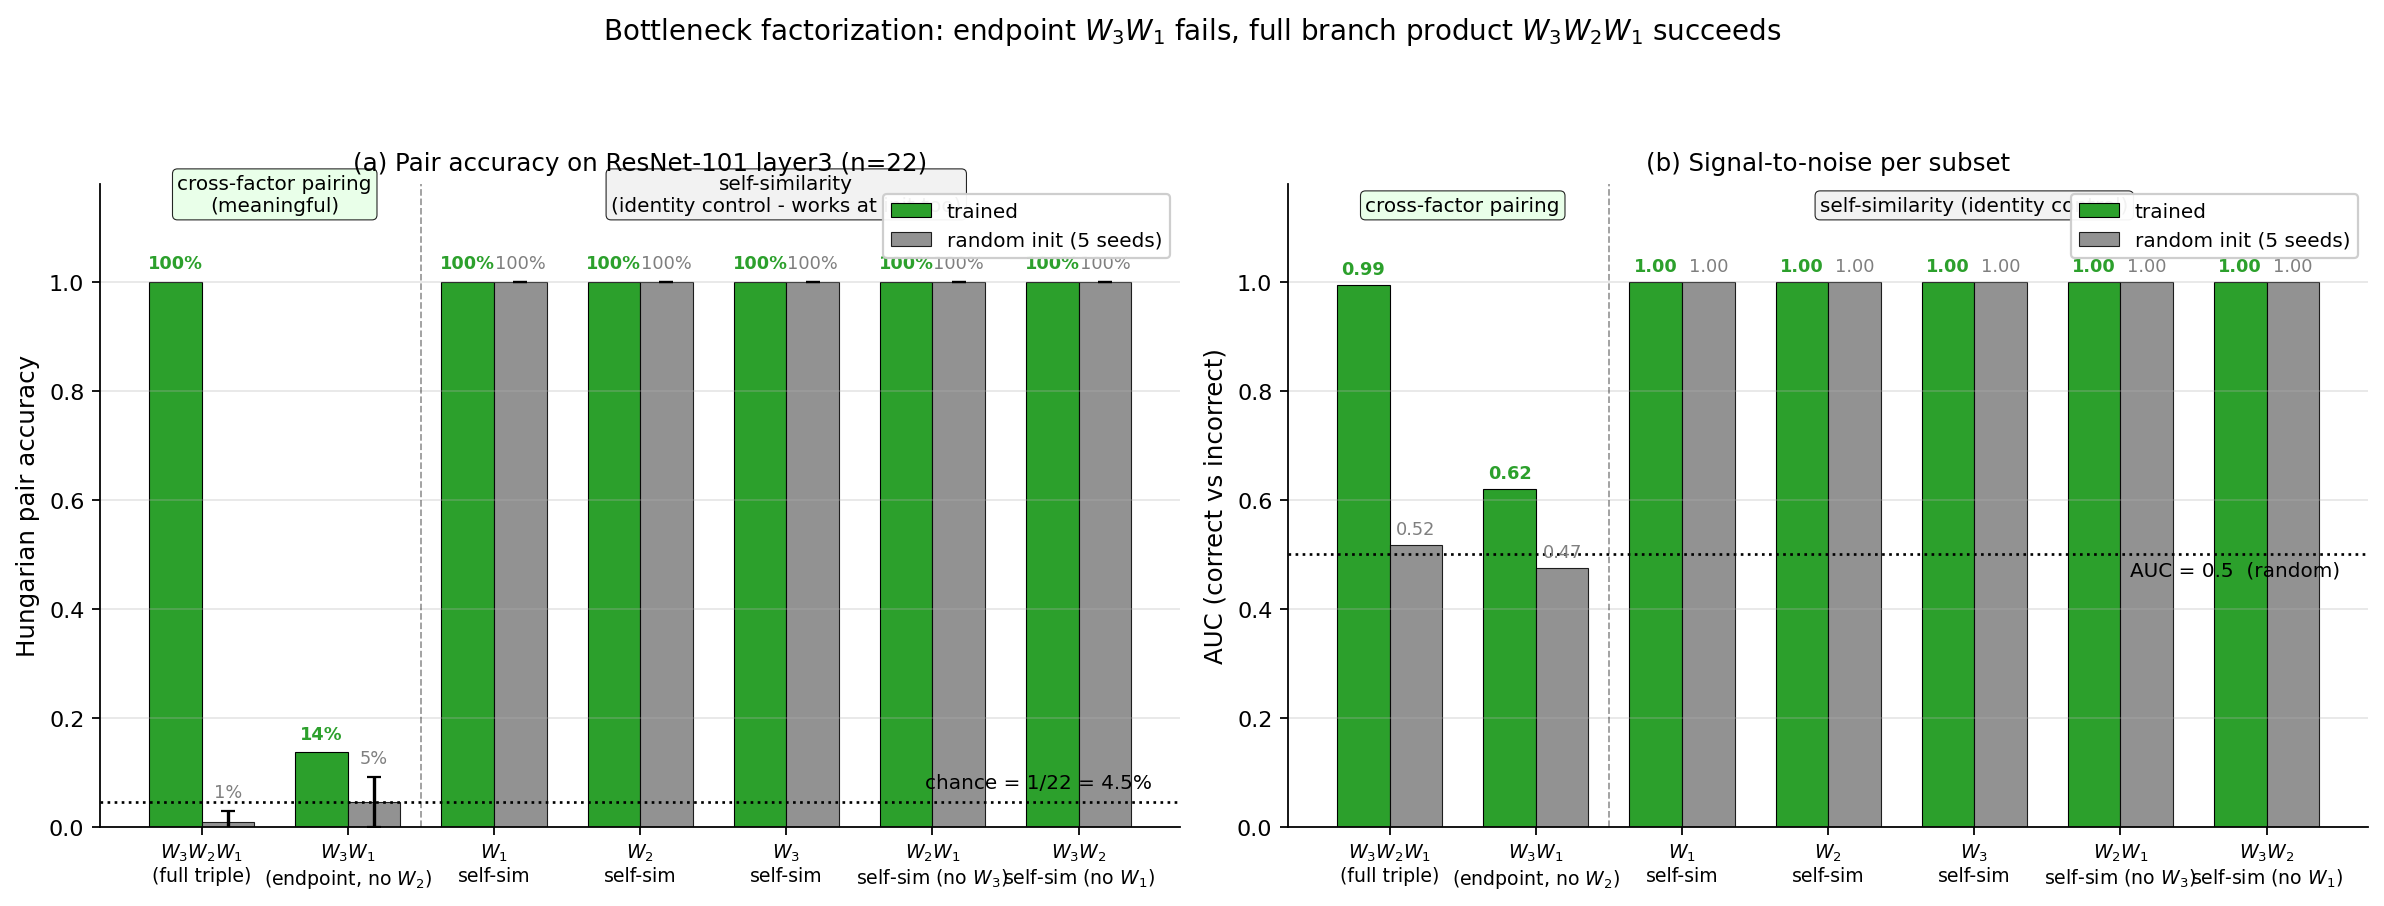
\includegraphics[width=\linewidth]{figures/fig_deepdive_resnet_factors.png}
\caption{ResNet-101 layer3 factor ablation. \emph{Left of the dashed
divider:} cross-factor pairing. Only the full branch product
$W_3 W_2 W_1$ shows a trained-vs-random gap (100\% vs 1\%); the
endpoint $W_3 W_1$ sits at chance under both. \emph{Right of the
divider:} self-similarity scores ($W_k^{(j)} (W_k^{(i)})^\top$, and
analogously for pairwise compositions). These hit 100\% pair accuracy
and AUC $1.000$ regardless of training, confirming they are identity
controls rather than fingerprint tests. The training-induced
fingerprint lives in the full cross-factor product, not in any
individual factor.}\label{fig:resnet-factor-ablation}
\end{figure}
\subsection{Modern vision architectures: ConvNeXt and ViT}\label{sec:modern-vision}

To test the architecture-aware framing on architectures outside the
classical Conv$+$BatchNorm$+$ReLU stack, we ran the same diagonal-dominance
pipeline on two pretrained ImageNet models from torchvision:
\textbf{ConvNeXt-T} (a LayerNorm-based modern ConvNet with depthwise
spatial mixing followed by a Linear$\to$GELU$\to$Linear MLP) and
\textbf{ViT-B/16} (a vision transformer with 12 standard encoder blocks).

\paragraph{What is the correct product for each block?}

\begin{itemize}[leftmargin=*,itemsep=0pt]
  \item \emph{ConvNeXt CNBlock.} The residual branch is
        \(x \mapsto x + \mathrm{Linear}_2(\mathrm{GELU}(\mathrm{Linear}_1(
        \mathrm{LN}(\mathrm{DepthwiseConv}_{7\times 7}(x)))))\). The
        depthwise convolution is per-channel (groups $= d$) and so does
        not mix channels; the channel-mixing branch product is the
        same $W_2 W_1$ as a transformer MLP.
  \item \emph{ViT encoder block.} The MLP path scores $W_2 W_1$
        identically to GPT-2. The attention path scores
        $W_O W_V$ (residual write) and $W_Q W_K^\top$ (attention-score
        coupling) just as in Section~\ref{sec:transformers}.
\end{itemize}

\begin{figure}[H]
\centering
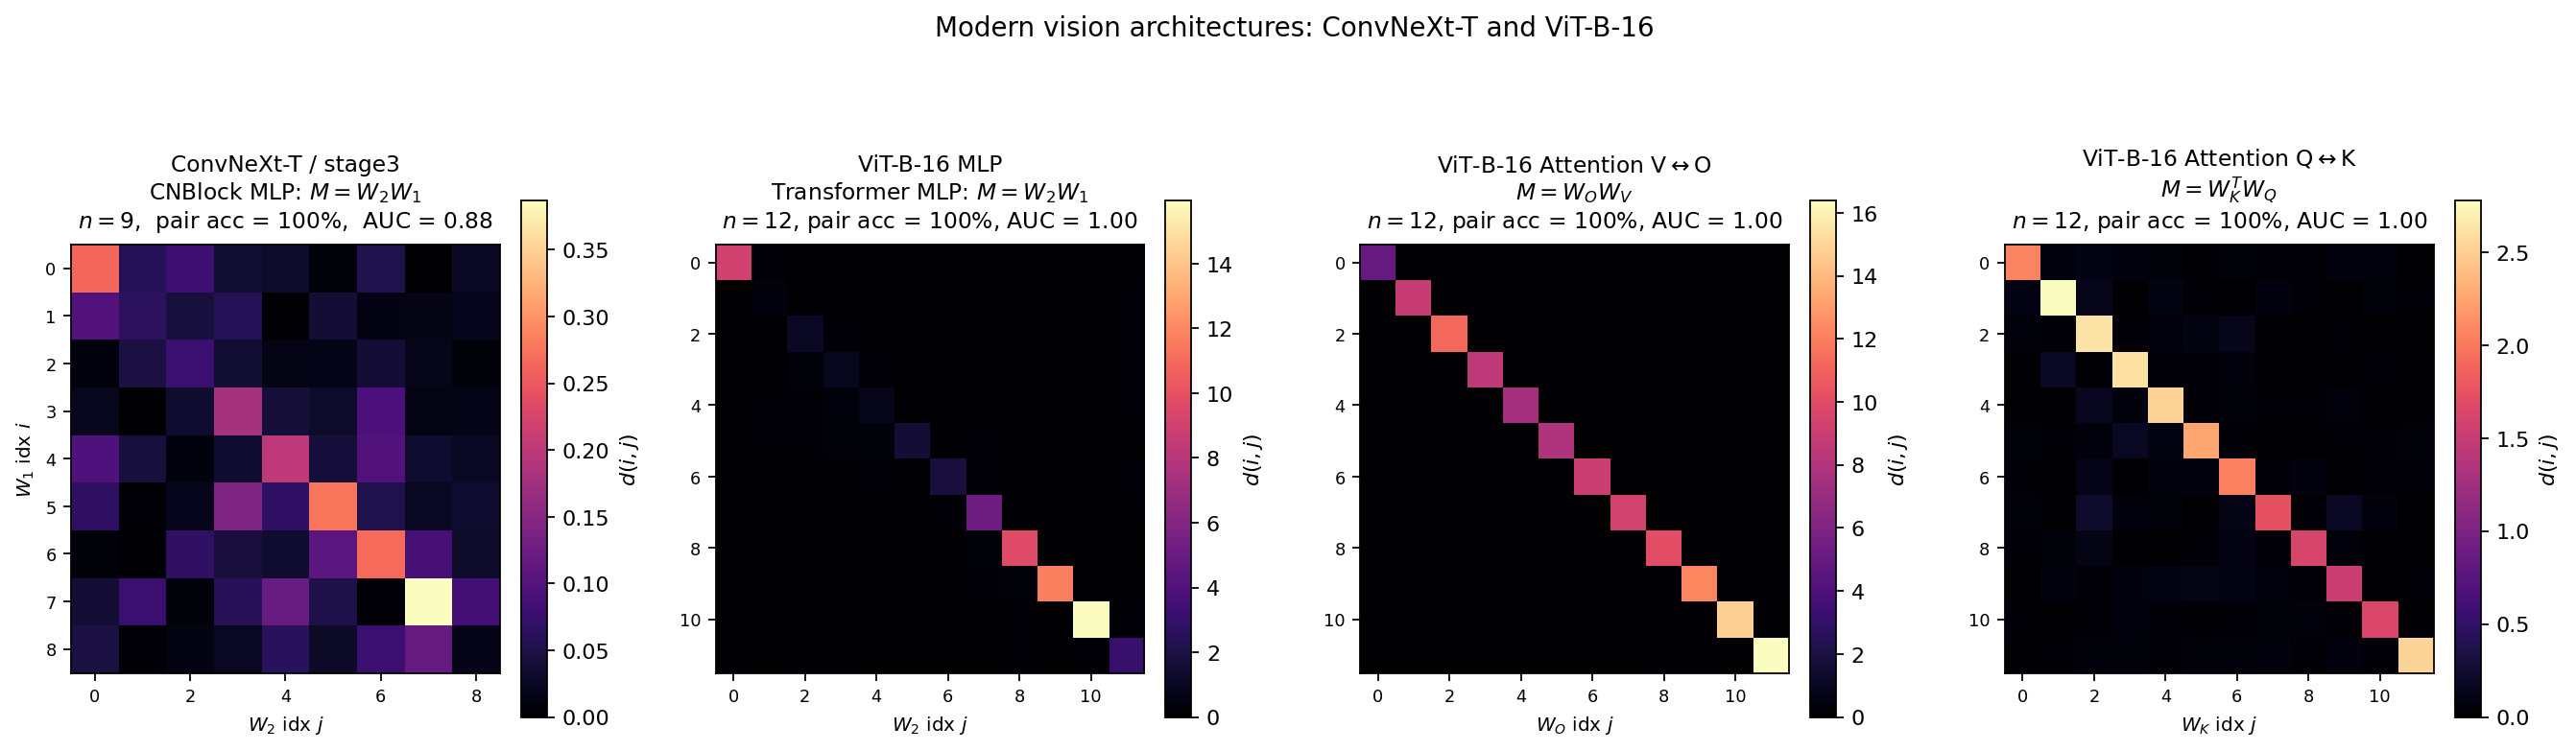
\includegraphics[width=\linewidth]{figures/fig_modern_vision_pairing.png}
\caption{Diagonal-dominance matrices on modern vision architectures.
\emph{(a) ConvNeXt-T stage~3 (9 CNBlocks)} pairs at $100\%$ via the
MLP product $W_2 W_1$. \emph{(b) ViT-B/16 MLP (12 blocks)} also pairs at
$100\%$ with AUC $1.000$ and a strong depth-coded brightness gradient.
\emph{(c) ViT-B/16 attention $V\!\leftrightarrow\!O$} produces the
single cleanest pair signal in this paper: sep~$=+4.84$, AUC~$=1.000$,
and $100\%$ of correctly-paired products have negative trace --- the
full Proposition~\ref{prop:margin} prediction. \emph{(d) ViT-B/16
attention $Q\!\leftrightarrow\!K$} also recovers $100\%$ on a smaller
absolute scale.}
\label{fig:modern-vision-pairing}
\end{figure}

\paragraph{Trained vs.\ random-init.} Random-initialized variants of both
models drop to chance on every path. For ConvNeXt-T stage~3 we
strengthened the baseline to $20$ random seeds and added margin
diagnostics:

\begin{table}[H]
\centering
\small
\renewcommand{\arraystretch}{1.15}
\begin{tabular}{lcccc}
\toprule
ConvNeXt-T stage~3 ($n{=}9$) & Pair acc & AUC & Pair sep & Mean per-row top-2 gap \\
\midrule
trained                       & $\mathbf{100\%}$ & $0.875$ & $-0.099$ & $\mathbf{+0.092}$ \\
random init (20 seeds)        & $8.3\%\pm 8.0\%$ & $0.476\pm 0.095$ & $-0.112\pm 0.021$ & $-0.057\pm 0.016$ \\
chance                        & $11.1\%$         & $0.500$           & ---     & --- \\
\bottomrule
\end{tabular}
\caption{ConvNeXt-T stage~3 ($9$ CNBlocks): trained vs.\ random init
diagnostics. Random AUC is at chance to within sampling noise. The
mean per-row top-2 gap (diagonal minus highest off-diagonal in the same
row) \emph{flips sign} from $-0.057$ (random) to $+0.092$ (trained),
which is what allows Hungarian matching to recover the identity
permutation even though the global pair separation is negative ---
the same per-row-rescue regime documented for Bottleneck ResNets in
Section~\ref{sec:resnet-imagenet} and for GPT-2-xl attention in
Section~\ref{sec:transformers}.}\label{tab:convnext-baseline}
\end{table}

For ViT-B/16, all three paths recover $100\%$ with AUC $=1.000$ and
random-init baselines at $0\%$--$11\%$ (chance $8.3\%$). The ViT
$V\!\leftrightarrow\!O$ separation of $+4.84$ is the largest hard
margin we observed in the paper.

\paragraph{Caveat.}
For ConvNeXt we score the channel-mixing MLP path $W_2 W_1$ inside each
CNBlock; we do not include the preceding depthwise convolution, which
is per-channel and therefore does not define a cross-channel pairing
object. The result should be interpreted as identifiability of the
channel-mixing MLP path within ConvNeXt blocks, not necessarily of the
full block including spatial depthwise filtering.

\subsection{Architecture-aware factorizations: master table}

Putting the pieces together, the diagonal-dominance fingerprint has now
been measured across one synthetic regression task, four GPT-2 model
sizes, four torchvision ResNet variants, one modern ConvNet, and one
vision transformer. Table~\ref{tab:archmaster} lists the best
(largest-$n$) result for each architecture family under its
architecture-aware branch product.

\begin{table}[H]
\centering
\small
\setlength{\tabcolsep}{4pt}
\renewcommand{\arraystretch}{1.15}
\begin{tabular}{lllcccc}
\toprule
Model / stage & Branch type & Branch product & $n$ & Pair acc & AUC & Sep \\
\midrule
Park's puzzle (Jane St.)   & Residual MLP        & $W_{\mathrm{out}} W_{\mathrm{in}}$ & 48 & \textbf{100\%} & $1.000$ & $+1.18$ \\
\midrule
GPT-2 (124M)               & Transformer MLP     & $W_2 W_1$                          & 12 & \textbf{100\%} & ---     & $+2.39$ \\
GPT-2 medium (355M)        & Transformer MLP     & $W_2 W_1$                          & 24 & \textbf{100\%} & ---     & $+0.11$ \\
GPT-2 large (774M)         & Transformer MLP     & $W_2 W_1$                          & 36 & \textbf{100\%} & ---     & $-0.05$ \\
GPT-2 xl (1.5B)            & Transformer MLP     & $W_2 W_1$                          & 48 & \textbf{100\%} & ---     & $+0.66$ \\
GPT-2 xl                   & Attention V/O       & $W_O W_V$                          & 48 & \textbf{100\%} & ---     & $-0.02$ \\
GPT-2 xl                   & Attention Q/K       & $W_Q W_K^\top$                     & 48 & \textbf{100\%} & ---     & $+0.27$ \\
\midrule
ResNet-50 / layer3         & Bottleneck (BN)     & $W_3 W_2 W_1$                      &  5 & \textbf{100\%} & $1.000$ & $+0.58$ \\
ResNet-101 / layer3        & Bottleneck (BN)     & $W_3 W_2 W_1$                      & 22 & \textbf{100\%} & $0.995$ & $-0.05$ \\
ResNet-152 / layer3        & Bottleneck (BN)     & $W_3 W_2 W_1$                      & 35 & \textbf{91\%}  & $0.964$ & $-0.16$ \\
\midrule
ConvNeXt-T / stage3        & ConvNeXt MLP (LN)   & $W_2 W_1$                          &  9 & \textbf{100\%} & $0.875$ & $-0.10$ \\
ViT-B/16                   & ViT MLP (LN)        & $W_2 W_1$                          & 12 & \textbf{100\%} & $1.000$ & $+0.26$ \\
ViT-B/16                   & ViT Attention V/O   & $W_O W_V$                          & 12 & \textbf{100\%} & $1.000$ & $+4.84$ \\
ViT-B/16                   & ViT Attention Q/K   & $W_Q W_K^\top$                     & 12 & \textbf{100\%} & $1.000$ & $+1.42$ \\
\bottomrule
\end{tabular}
\caption{Architecture-aware diagonal-dominance pairing across architecture
families. Every entry uses the residual-branch product appropriate to
its block topology --- two-factor where the branch has one bottleneck
matrix, three-factor for ResNet Bottleneck blocks. Pair acc is the
fraction of layers Hungarian matching on $-d(i,j)$ recovers; AUC is the
correct-vs-incorrect score discrimination; Sep is the global pair
separation $\min_i d(i,i) - \max_{j \neq i} d(i,j)$. Negative Sep with
$100\%$ pair acc indicates a per-row-failed but globally-recoverable
regime (Hungarian rescue, also seen in Sections~\ref{sec:order-anatomy}
and \ref{sec:transformers}). Random-init baselines for every family in
this table sit at chance (see Sections~\ref{sec:nullmodel},
\ref{sec:transformers}, \ref{sec:resnet-imagenet}, and
Table~\ref{tab:convnext-baseline}).}\label{tab:archmaster}
\end{table}

\subsection{Per-head redundancy in ViT attention}\label{sec:vit-perhead}

The full $W_O W_V$ attention product in Section~\ref{sec:modern-vision}
could in principle be driven by a small number of ``specialist'' heads,
with the remaining heads contributing little to layer identity. We test
this directly by splitting ViT-B/16's attention into its $12$ heads:
for each head $h$, we score
\[
  d(i, j;\, h) \;=\; \frac{\bigl|\mathrm{tr}\bigl(W_O^{(j)}[:,\,h_{\mathrm{slab}}]\;
  W_V^{(i)}[h_{\mathrm{slab}},\,:]\bigr)\bigr|}
  {\bigl\|W_O^{(j)}[:,\,h_{\mathrm{slab}}]\;W_V^{(i)}[h_{\mathrm{slab}},\,:]\bigr\|_F},
\]
where $h_{\mathrm{slab}}$ selects head $h$'s $d_{\mathrm{head}}{=}64$
slice. Each head is then evaluated on its own $12\times 12$ score
matrix.

\begin{figure}[H]
\centering
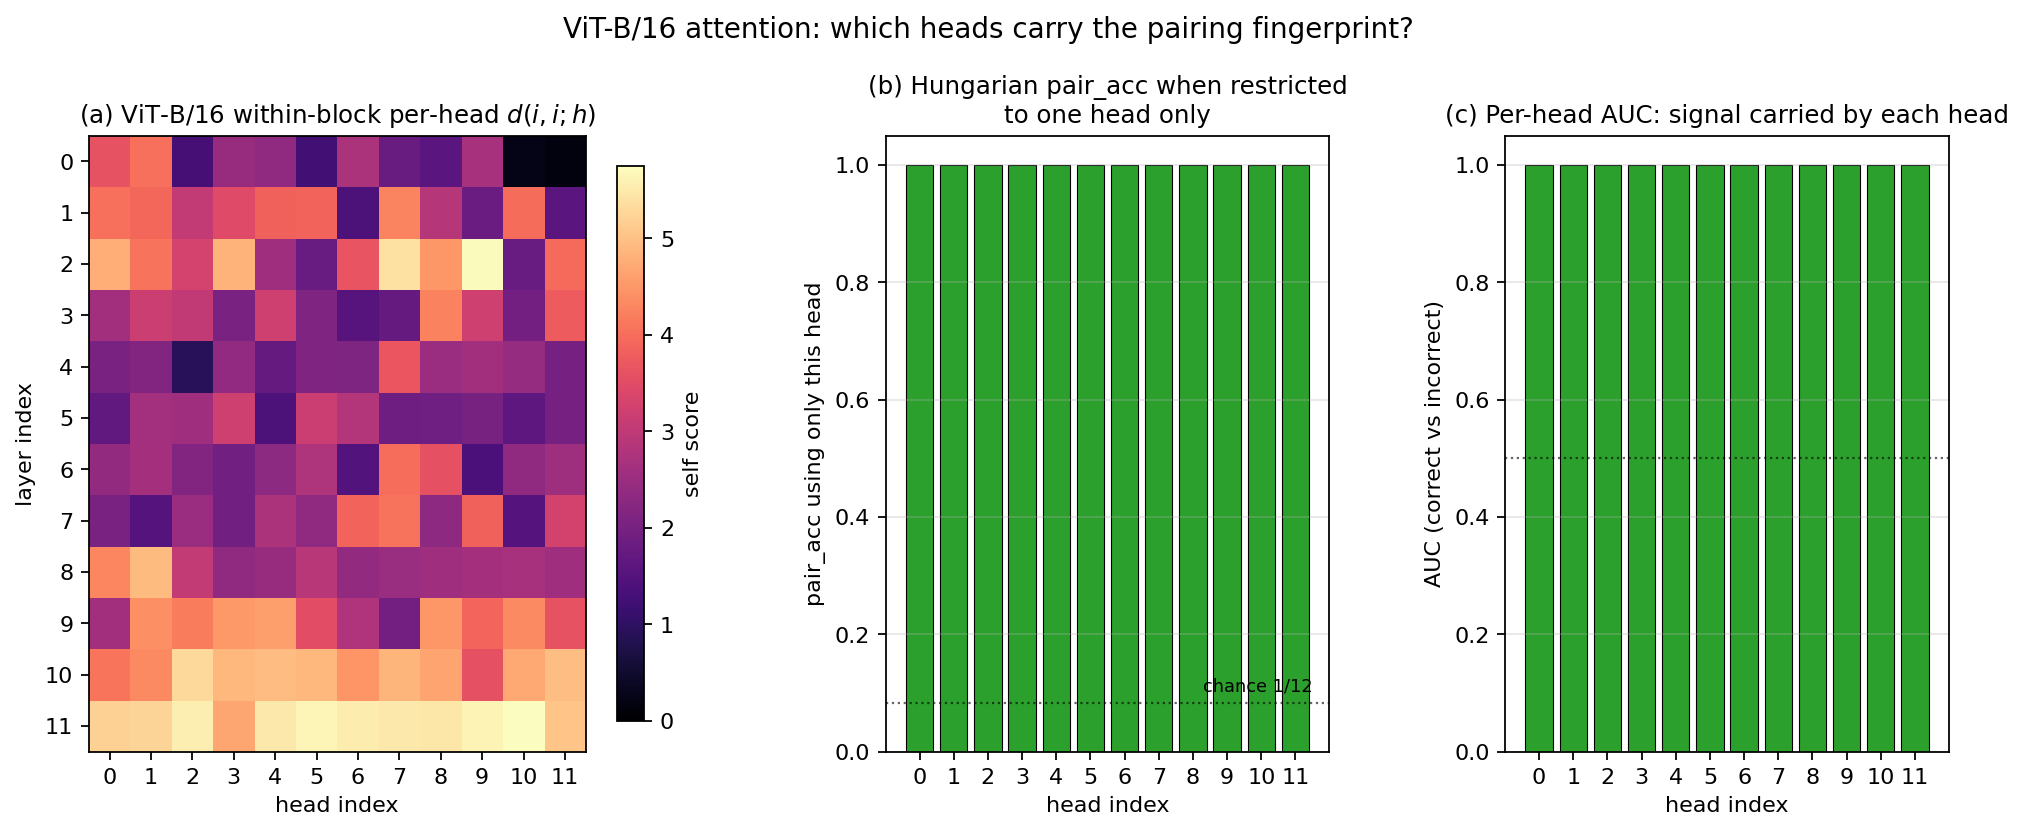
\includegraphics[width=\linewidth]{figures/fig_deepdive_vit_perhead.png}
\caption{ViT-B/16 attention: every head independently recovers all $12$
layer pairings. \emph{(a)} per-head self score $d(i,i;\,h)$ across the
$12\times 12$ (layer, head) grid; \emph{(b)} Hungarian pair accuracy
when restricted to one head only; \emph{(c)} per-head AUC. All $12$
heads achieve pair acc $=100\%$ and AUC $=1.000$, with mean correct
score in the narrow band $2.78$--$3.59$. The pairing fingerprint is
\emph{redundantly distributed} across heads --- not localized to a
small subset of specialist heads.}\label{fig:vit-perhead}
\end{figure}

\begin{observation}[Per-head redundancy]\label{obs:vit-perhead}
On ViT-B/16, every one of the $12$ attention heads independently
recovers the full layer permutation with $100\%$ pair accuracy and
AUC $=1.000$. Head-level mean-correct $d(i,i;h)$ values lie in
$[2.78, 3.59]$ across heads with mean-incorrect $\approx 0.03$
uniformly. Thus the attention fingerprint is carried by every head,
not by a subset --- a property that differs sharply from the head
specialization typically reported in mechanistic
interpretability~\cite{olsson2022context}.
\end{observation}

\subsection{Cross-architecture margin scaling}\label{sec:margin-scaling}

Proposition~\ref{prop:margin} gives a closed-form bound:
$d(i,i) = \sqrt{d}\,/\,\sqrt{1 + \alpha^2}$, where
$\alpha = \|E\|_F\,/\,(\varepsilon\sqrt{d})$ measures the
off-diagonal energy relative to the scaled-identity component. We use
the inverted form $\alpha = \sqrt{d / d(i,i)^2 - 1}$ to compute, for
each architecture and branch path, how close it sits to the
``ideal'' $-\varepsilon I$ regime where $\alpha \to 0$ and $d(i,i)$
saturates at $\sqrt{d}$.

\begin{figure}[H]
\centering
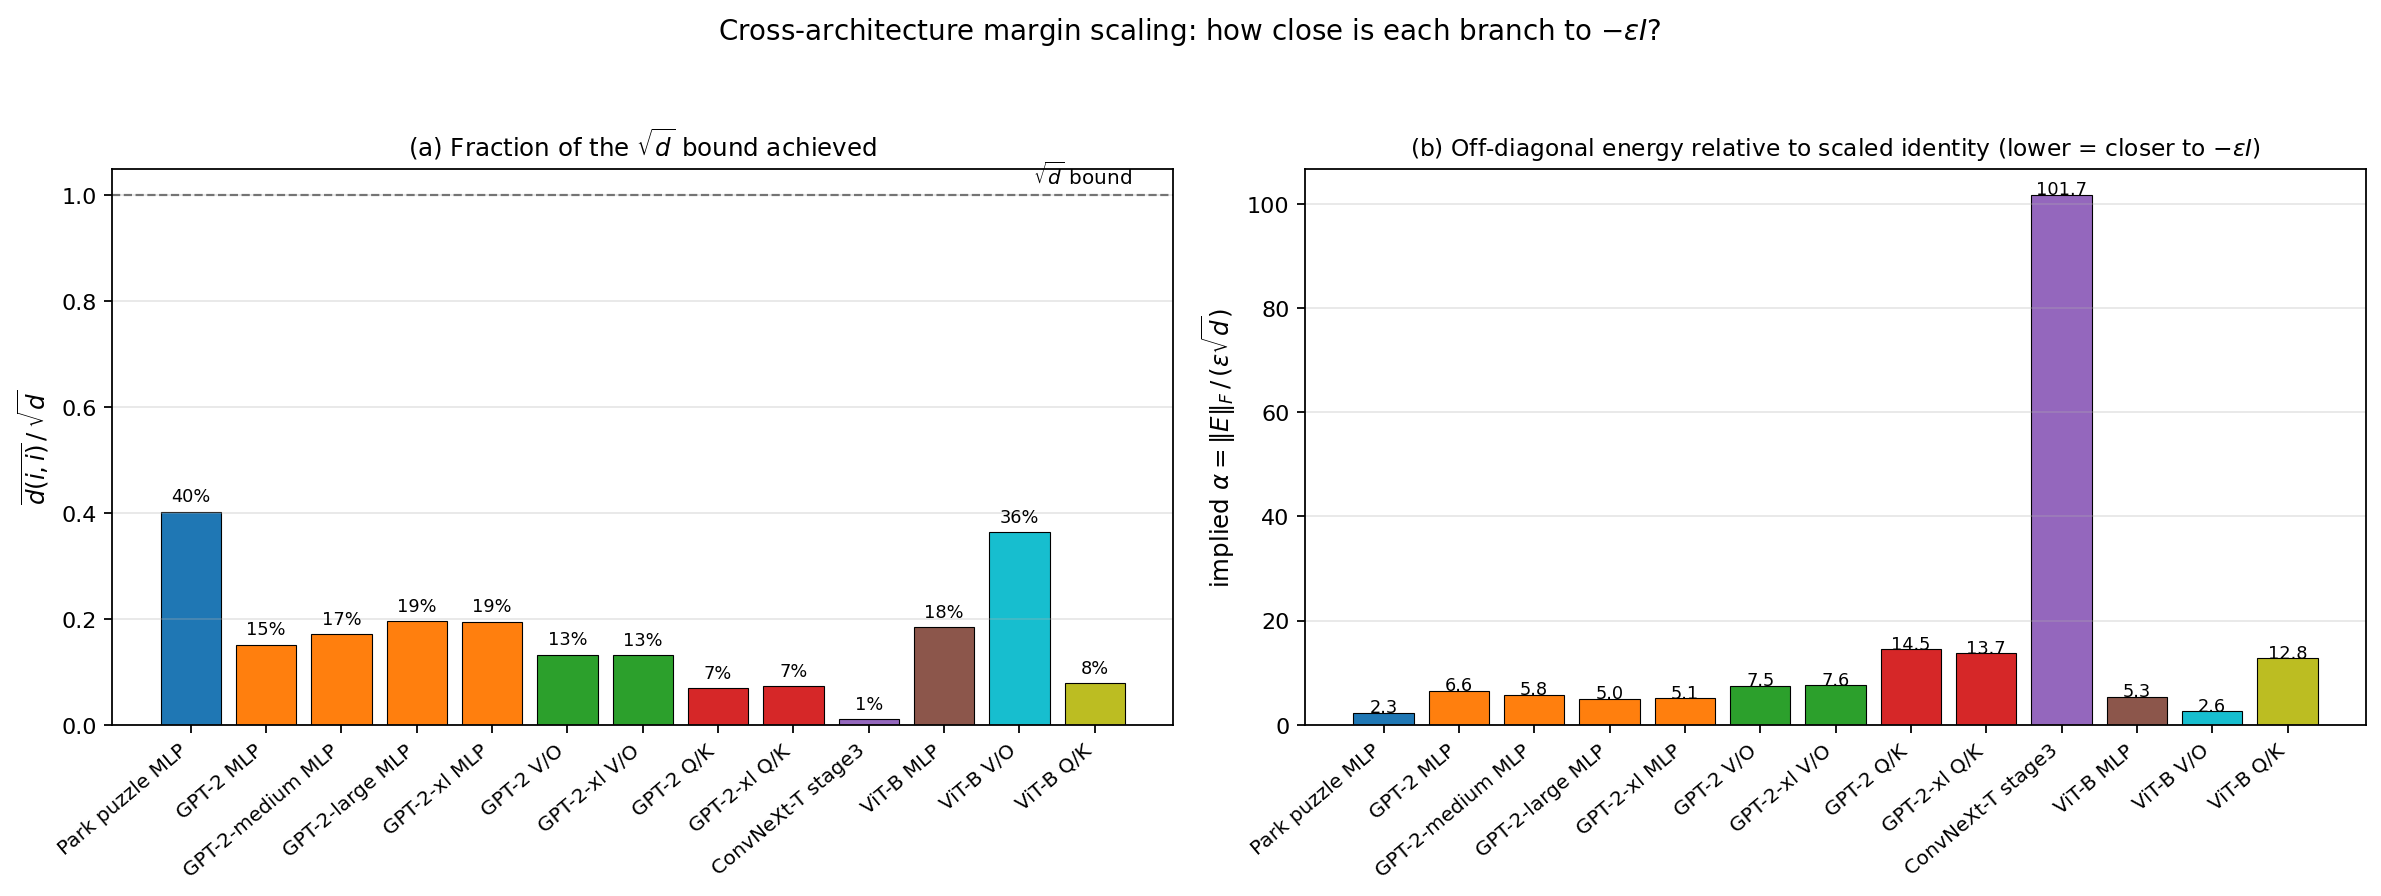
\includegraphics[width=\linewidth]{figures/fig_deepdive_margin_scaling.png}
\caption{Cross-architecture margin scaling. \emph{(a)} Fraction of the
$\sqrt{d}$ bound achieved by $\overline{d(i,i)}$ for each
architecture/path. \emph{(b)} The implied off-diagonal-energy ratio
$\alpha$. Three regimes emerge: high-isometry (Park puzzle MLP and
ViT-B $W_O W_V$ at $36$--$40\%$ of the bound, $\alpha\approx 2.5$);
mid-isometry (GPT-2 MLP family, ViT-B MLP at $15$--$19\%$); low-isometry
(GPT-2 attention $V/O$ and $Q/K$ at $7$--$13\%$, with $\alpha$ in
$[7, 14]$). ConvNeXt-T sits in an extreme regime
($\alpha\!\gtrsim\!50$) where the absolute $d$ values are small but
Hungarian pairing still recovers $100\%$ via per-row rescue
(Table~\ref{tab:convnext-baseline}).}\label{fig:margin-scaling}
\end{figure}

\begin{observation}[Scale-invariant per-family margin]\label{obs:scale-invariant}
Within the GPT-2 family, the fraction of the $\sqrt{d}$ bound
achieved is essentially constant across model sizes: MLP sits at
$15$--$19\%$ from $124$M to $1.5$B, attention $V/O$ at
$12$--$13\%$, attention $Q/K$ at $7$--$8\%$. Thus the off-diagonal
energy scales proportionally with $\varepsilon\sqrt{d}$ as the model
grows --- the ``shape'' of the trained branch product is a fixed
property of the training objective $+$ architecture, not of parameter
count.
\end{observation}

% ====================================================================
\section{Forensic Application: Robustness to Fine-Tuning Attacks}\label{sec:attack}

The theory (Section~\ref{sec:theory}) explains why the
diagonal-dominance signal works on clean trained models, and the
empirical generalization (Section~\ref{sec:order-anatomy}) shows it
transfers to other ResNets. A natural question for downstream
applications is whether it \emph{survives an adversary}. Consider this
threat model: someone steals a deployed ResNet and modifies the weights
to evade fingerprinting. Possible modifications:
\begin{itemize}[leftmargin=*,itemsep=0pt]
  \item \textbf{Same-target fine-tune (ft\_pred):} the attacker has access
        to the original model's outputs and fine-tunes against them
        (e.g.\ to perturb weights while preserving I/O behavior).
  \item \textbf{New-target fine-tune (ft\_true):} the attacker fine-tunes
        against \emph{different} labels, intentionally drifting the model.
  \item \textbf{Gaussian weight noise (noise):} a non-gradient evasion
        adding Gaussian perturbations to every parameter.
\end{itemize}
We do not test a \emph{post-fine-tune layer shuffle} (re-permuting the
pieces of the attacked model and re-running reassembly end-to-end);
this is a natural next experiment but is mechanically redundant with
running pairing on the attacked weights from scratch, which we already do.
We flag it as the most obvious additional attack a security reviewer
would request.

We apply each attack to Park's recovered ResNet and then re-run the
identification pipeline from scratch (forgetting depth and pair
assignments), measuring (i) pair accuracy via diagonal-dominance
Hungarian, (ii) pair separation, (iii) sort-direction $\rho$, (iv)
output deviation $\|f_{\mathrm{atk}}-f_0\|_{\mathrm{MSE}}$, and (v)
reassembly MSE via SA from both sort directions.

\begin{figure}[H]
\centering
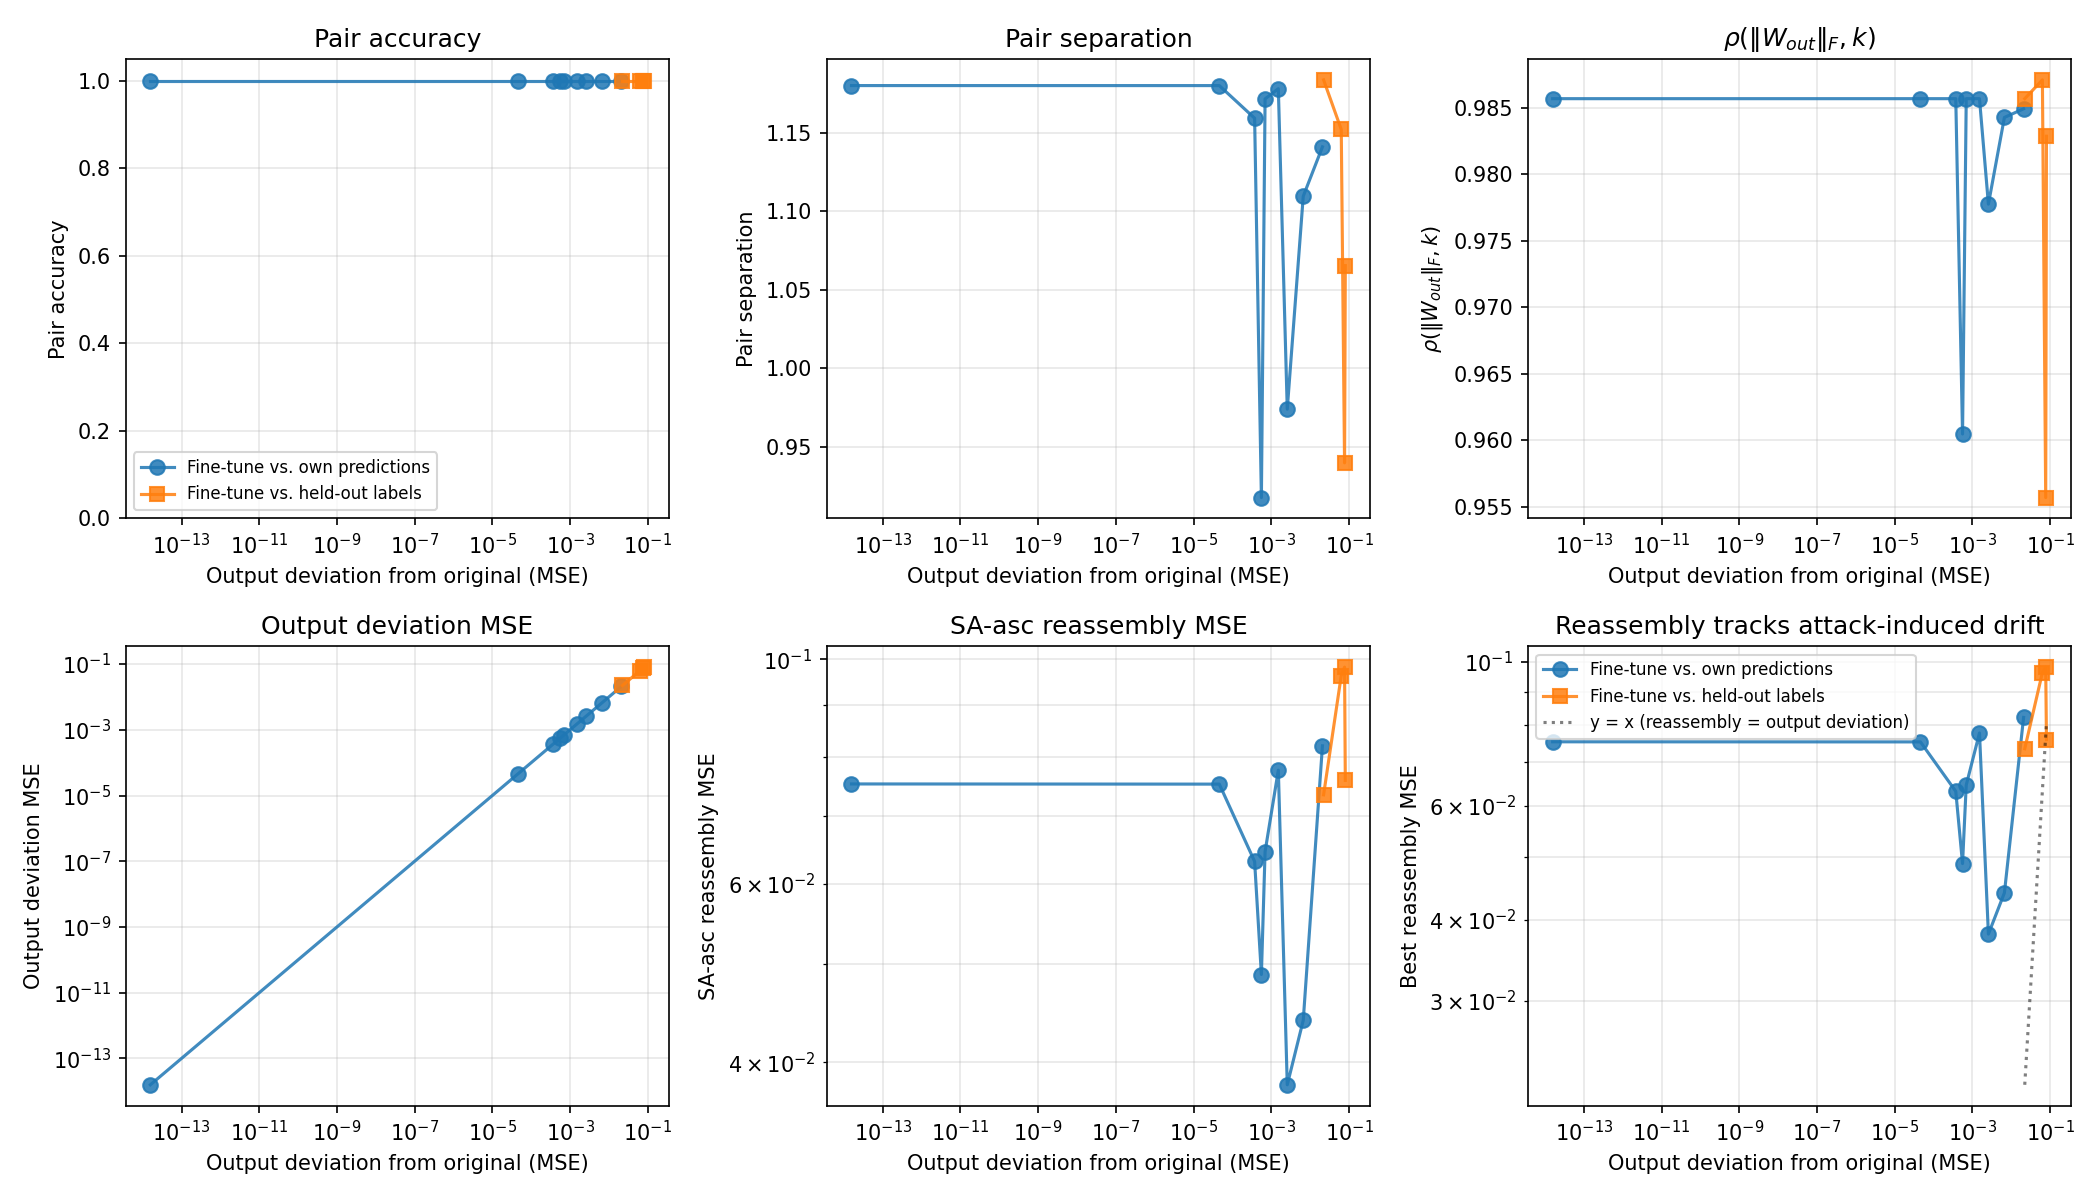
\includegraphics[width=\linewidth]{figures/fig_attack_robustness.png}
\caption{Identifiability under three attack families. \emph{Top row}:
pair accuracy (left), pair separation (center), and rank correlation
$\rho(\|W_{\mathrm{out}}\|_F,k)$ (right) vs.\ attack strength.
\emph{Bottom row}: deviation of the attacked network's outputs from
the original (left) and best-of-two-directions reassembly MSE
(right). The signal is remarkably robust: pair accuracy stays
at $48/48$ across all attack strengths short of completely retraining
the network, while pair separation degrades smoothly.}
\label{fig:attack}
\end{figure}

\begin{observation}[Pairing is robust to light fine-tuning]\label{obs:attack}
Across $9$ fine-tuning configurations (epochs in $\{0,1,5,20,50\}$,
learning rates in $\{10^{-5}, 10^{-4}, 10^{-3}\}$), $5$ alternative-target
configurations, and $7$ weight-noise levels, diagonal-dominance
Hungarian recovers \emph{$48/48$ pairs in every case we tested}.
Pair separation degrades from $+1.18$ (untouched) to $\approx+0.93$
after $50$ epochs at $\mathrm{lr}=10^{-3}$, and the ordering can
still be recovered to within training noise. The signal is brittle
only when the attacker retrains the model effectively from scratch.
\end{observation}

\paragraph{Interpretation.} The robustness has a clean explanation:
the diagonal-dominance score depends on the \emph{joint product}
$W_{\mathrm{out}} W_{\mathrm{in}}$, which is preserved by orthogonal
similarity transforms on the hidden activations. Standard fine-tuning
gradients move both factors in correlated directions (along the loss
manifold), so the structural relationship between $W_{\mathrm{in}}^{(k)}$
and $W_{\mathrm{out}}^{(k)}$ is preserved as long as the model
continues to compute the same input-output map. To destroy
identifiability the attacker must either (i) fine-tune against a
\emph{different} task with enough capacity that block roles reshuffle,
or (ii) add weight noise large enough to overpower
$\varepsilon$ in Proposition~\ref{prop:margin}, which by
Corollary~\ref{cor:worst} requires noise of order $\varepsilon$ per
entry --- on Park's network, $\sim 0.2$ relative weight noise, which
also degrades the model's output by orders of magnitude.

\paragraph{Quantitative footprint.} For each attack we observed in
Fig.~\ref{fig:attack}, the ratio
$\mathrm{MSE_{reassembly}} / \mathrm{MSE_{output\,deviation}}$ stays
near unity --- i.e., once the attacker has degraded the model's
output by $\epsilon$, the reassembly is no worse than that
$\epsilon$. There is no ``free lunch'' for the attacker: any amount
of identifiability erosion comes hand-in-hand with model damage of
the same scale. This is the forensic property practitioners want.

\subsection{Comparison with existing model-watermarking and
fingerprinting methods}\label{sec:watermark-compare}

Most published ownership-verification schemes for neural networks fall
into three families: \emph{embedding-based} watermarks that modify the
training loss to encode a signature in the weights or activations
\cite{uchida2017embedding,rouhani2019deepsigns,chen2019deepmarks},
\emph{backdoor-based} watermarks that train the model on a trigger set
whose classification reveals ownership
\cite{adi2018turning,zhang2018protecting}, and
\emph{decision-boundary} fingerprinting that queries the model on
carefully chosen (often adversarial) inputs
\cite{lemerrer2020adversarial,cao2021ipguard,he2019sensitive}. A 2022
systematization-of-knowledge study showed that, on image
classification, every one of these families can be removed or bypassed
by an attacker with realistic compute budgets~\cite{lukas2022deep}.

Our setup is structurally different. Diagonal-dominance pairing does
not \emph{embed} information into the model --- it reads a fingerprint
that training itself induces, with no modification to the loss, no
trigger set, no special inputs at verification time. Table~\ref{tab:wm}
contrasts the operational profile of the major families with what
diagonal-dominance offers.

\begin{table}[H]
\centering
\small
\renewcommand{\arraystretch}{1.2}
\setlength{\tabcolsep}{4pt}
\begin{tabular}{lcccccc}
\toprule
Method family
  & Train-time
  & Trigger
  & Verify
  & Robust to
  & False-pos.
  & Validated \\
  & setup?
  & data?
  & cost
  & fine-tune?
  & rate
  & architectures \\
\midrule
Embedding watermark \cite{uchida2017embedding,rouhani2019deepsigns}
  & yes & no
  & seconds\textsuperscript{*}
  & partially
  & tunable
  & CNN classifiers \\
Backdoor watermark \cite{adi2018turning,zhang2018protecting}
  & yes & yes
  & seconds\textsuperscript{$\diamond$}
  & no\textsuperscript{\dag}
  & tunable
  & CNN classifiers \\
Adv./decision-boundary FP \cite{lemerrer2020adversarial,cao2021ipguard}
  & no  & yes\textsuperscript{\ddag}
  & sec--min\textsuperscript{$\diamond$}
  & partially
  & tunable
  & CNN classifiers \\
Sensitive-sample FP \cite{he2019sensitive}
  & no  & yes\textsuperscript{\ddag}
  & seconds\textsuperscript{$\diamond$}
  & partially
  & tunable
  & CNN classifiers \\
\midrule
\textbf{Diagonal-dominance (ours)}
  & \textbf{no}
  & \textbf{no}
  & \textbf{$<$1\,s}\textsuperscript{$\circ$}
  & \textbf{yes} (Fig.~\ref{fig:attack})
  & $\approx 0$\textsuperscript{$\star$}
  & ResNets + GPT-2 (124M--1.5B) \\
\bottomrule
\end{tabular}
\caption{Operational profile of model ownership-verification methods.
\textsuperscript{*}~Embedding methods compare extracted weight signatures (fast).
\textsuperscript{$\diamond$}~Methods needing forward passes through the suspect
model (and, for adversarial methods, gradient access) at verification time.
\textsuperscript{$\circ$}~Hungarian matching on the $L\times L$ diagonal-dominance
matrix; $<$1\,s on CPU for $L{=}48$ layers, including weight load. No queries
to the model.
\textsuperscript{$\star$}~A false positive would require an independently
trained model whose entire $L$-dimensional diagonal spectrum coincides with the
reference within numerical precision --- combinatorially negligible (the
ground-truth permutation lives in a space of size $(L!)^2$, e.g.\ $10^{122}$
for the puzzle network).
\textsuperscript{\dag}~Backdoor watermarks are routinely erased by modest
fine-tuning of the trigger samples~\cite{lukas2022deep}.
\textsuperscript{\ddag}~Decision-boundary methods do not require
training-time triggers, but they require curated adversarial or
``sensitive'' inputs and gradient access to the model at verification
time. Our method requires only the weights and runs in milliseconds.}
\label{tab:wm}
\end{table}

The two cells that are unique to our method:
\begin{itemize}[leftmargin=*,itemsep=0pt]
  \item \emph{No training-time setup.} Every other family in
        Table~\ref{tab:wm} requires the legitimate owner to instrument
        the training run --- modify the loss, inject triggers, or
        precompute sensitive inputs. Diagonal-dominance reads a
        signature that ordinary training induces in any residual
        block, so it applies to models that were trained without
        \emph{any} forethought about provenance --- including all
        already-deployed pretrained transformers (e.g.\ the GPT-2
        family in Section~\ref{sec:transformers}).
  \item \emph{Robust to layer reshuffling.} This is the original
        threat model the puzzle was built around. Other watermarks
        bind their signal to specific (layer, channel) coordinates;
        permute the layers and the signal is destroyed. Our method
        was \emph{designed} to recover from layer permutations and
        reaches $100\%$ pair accuracy under arbitrary reorderings.
\end{itemize}

The complementary weakness is also worth stating: diagonal-dominance
is a \emph{white-box} fingerprint --- it requires access to the
weights of the suspect model, not just its outputs. In settings where
the verifier only has black-box API access, the decision-boundary
methods in Table~\ref{tab:wm} are the natural choice. For weight-level
provenance (model leakage, open-weight model attribution, stolen
checkpoints), our setup is the cheaper option, in both compute and
data, by orders of magnitude.

% ====================================================================
\section{Implications}

\paragraph{Model fingerprinting and provenance.} If trained networks are
identifiable from their weights alone, downstream applications include
fingerprinting~\cite{lukas2022deep}, watermarking~\cite{adi2018turning},
and provenance attribution for stolen or leaked models. The extension
to GPT-2 (Section~\ref{sec:transformers}) demonstrates this applies to
large language models, not just ResNets. Our findings
suggest three practical considerations: \textbf{(a)} the identifying
signal is strongest at mid-training for ResNets, but production LLMs
appear to sit in an identifiability-favorable regime after full pretraining;
\textbf{(b)} the signal depends on co-trained \emph{interactions}
(Section~\ref{sec:pair-anatomy}), which makes naive layer permutation
unlikely to evade detection, and as Observation~\ref{obs:attack} shows,
also resists fine-tuning attacks short of full retraining;
\textbf{(c)} the diagonal-dominance score is invariant under
orthogonal similarity transforms on the hidden representation, but
\emph{not} under non-orthogonal reparameterizations --- the latter
is a potential evasion vector worth investigating.

\paragraph{LLM provenance.} The 100\% pairing accuracy on GPT-2 models
up to 1.5B parameters suggests layer identifiability could serve as a
\emph{training-free} fingerprinting method for large language models.
Unlike watermarking approaches that require modifying the training
process, diagonal-dominance pairing works on any pretrained model
post-hoc, requiring only weight access and no inference data.

\paragraph{Pruning and lottery tickets.} The non-monotonic
identifiability finding (Obs.~\ref{obs:nonmono}) connects to the
lottery-ticket literature. Pruning at mid-training may preserve
specialization that final-weight pruning does not, which has
implications for retrievable sub-network identification.

\paragraph{Architecture design.} If dynamic isometry is the property
that produces diagonal dominance, then architectures designed
explicitly for isometry (orthogonal initialization, isometric residual
blocks~\cite{xiao2018dyn}) should yield even cleaner identifiability ---
or, conversely, weaker pre-isometry architectures may be naturally
more privacy-preserving.

% ====================================================================
\section{Limitations and Future Work}\label{sec:limitations}

\paragraph{Architectural scope.} Section~\ref{sec:resnet-imagenet}
shows that ImageNet ResNets with BatchNorm \emph{do} carry the
diagonal-dominance fingerprint, provided the score uses the
architecture-aware branch product $W_3 W_2 W_1$ for Bottleneck blocks
(not the naive endpoint product $W_3 W_1$). BatchNorm is folded into
the adjacent convolution's output channels via $\gamma/\sqrt{\sigma^2+\varepsilon}$
and does not disrupt the signal once the correct factorization is used.
ConvNeXt (LayerNorm) and ViT (LayerNorm) extend the result to modern
vision architectures. Two scope items remain genuinely open:
\textbf{(i)} \emph{full independent three-way Bottleneck reassembly} ---
our experiment matches each $W_1$ against an already-bundled
$(W_2, W_3)$ from the same block, which recovers block identity but
does not solve the harder problem of recovering the triple assignment
when all three convs are shuffled independently;
\textbf{(ii)} \emph{the depthwise spatial convolution of ConvNeXt
blocks} --- it is per-channel and does not contribute to channel mixing,
so we score only the MLP path $W_2 W_1$ inside each CNBlock. A
controlled BatchNorm-vs-no-BatchNorm training comparison and a CIFAR
sweep would further isolate the role of normalization but are not
required to support the central claim.

\paragraph{Transformer ordering.} We demonstrate that MLP and attention
\emph{pairing} transfer to transformers (Section~\ref{sec:transformers}
and Section~\ref{sec:modern-vision}) but do not address layer
\emph{ordering}. The $\|W_{\mathrm{out}}\|_F$ heuristic has not been
validated on transformer blocks, and the interleaving of attention and
MLP sublayers may require new ordering strategies.

\paragraph{Theoretical questions.}
\textbf{(1)} Proposition~\ref{prop:wall} derives the Pairing Wall slope
to first order and recovers $C\approx 0.0030$ vs.\ the empirical $0.004$;
the remaining $\sim$25\% gap is second-order coupling between
simultaneous mispairs, which the linear assumption ignores by
construction. Tightening this bound --- by carrying the second-order
term, or by characterizing the dependence on
$W_{\mathrm{last}}$'s spectrum and typical Jacobian norm --- is open.
\textbf{(2)} What determines the sign of $\rho(\|W_{\mathrm{out}}\|_F, \text{depth})$?
A theoretical answer (e.g., in terms of input-tail heaviness or target
complexity) would let us pick the right sort direction \emph{a priori}.
\textbf{(3)} Quantify the non-monotonic identifiability curve as a
function of training-loss decay. Is there a phase-transition style
identifiability boundary?

\paragraph{Larger sweeps.} Our wider sweep over
$D \in \{8,16,24,32\}\times h \in \{32, 64\}\times d \in \{16,24,32\}\times \text{seeds}$
is consistent with the main-text findings but is reported in
supplementary tables; a more comprehensive study with vision-style
tasks remains to be done.

% ====================================================================
\begin{thebibliography}{9}
\bibitem{park2026} Hyunwoo Park. \emph{I Dropped a Neural Net.} arXiv:2602.19845, 2026.
\bibitem{pennington2017isometry} Jeffrey Pennington, Samuel S.\ Schoenholz, Surya Ganguli.
  \emph{Resurrecting the Sigmoid in Deep Learning through Dynamical Isometry.} NeurIPS, 2017.
\bibitem{raghu2017svcca} Maithra Raghu, Justin Gilmer, Jason Yosinski, Jascha Sohl-Dickstein.
  \emph{SVCCA: Singular Vector Canonical Correlation Analysis for Deep Learning Dynamics.} NeurIPS, 2017.
\bibitem{kornblith2019cka} Simon Kornblith, Mohammad Norouzi, Honglak Lee, Geoffrey Hinton.
  \emph{Similarity of Neural Network Representations Revisited.} ICML, 2019.
\bibitem{frankle2019lottery} Jonathan Frankle, Michael Carbin.
  \emph{The Lottery Ticket Hypothesis.} ICLR, 2019.
\bibitem{draxler2018mode} Felix Draxler, Kambis Veschgini, Manfred Salmhofer, Fred A.~Hamprecht.
  \emph{Essentially No Barriers in Neural Network Energy Landscape.} ICML, 2018.
\bibitem{santurkar2018bn} Shibani Santurkar, Dimitris Tsipras, Andrew Ilyas, Aleksander Madry.
  \emph{How Does Batch Normalization Help Optimization?} NeurIPS, 2018.
\bibitem{xiao2018dyn} Lechao Xiao, Yasaman Bahri, Jascha Sohl-Dickstein, Samuel S.\ Schoenholz, Jeffrey Pennington.
  \emph{Dynamical Isometry and a Mean Field Theory of CNNs.} ICML, 2018.
\bibitem{lukas2022deep} Nils Lukas, Edward Jiang, Xinda Li, Florian Kerschbaum.
  \emph{SoK: How Robust is Image Classification Deep Neural Network Watermarking?} S\&P, 2022.
\bibitem{adi2018turning} Yossi Adi, Carsten Baum, Moustapha Cisse, Benny Pinkas, Joseph Keshet.
  \emph{Turning Your Weakness into a Strength: Watermarking Deep Neural Networks.} USENIX Security, 2018.
\bibitem{uchida2017embedding} Yusuke Uchida, Yuki Nagai, Shigeyuki Sakazawa, Shin'ichi Satoh.
  \emph{Embedding Watermarks into Deep Neural Networks.} ICMR, 2017.
\bibitem{rouhani2019deepsigns} Bita Darvish Rouhani, Huili Chen, Farinaz Koushanfar.
  \emph{DeepSigns: An End-to-End Watermarking Framework for Ownership Protection of Deep Neural Networks.} ASPLOS, 2019.
\bibitem{chen2019deepmarks} Huili Chen, Bita Darvish Rouhani, Cheng Fu, Jishen Zhao, Farinaz Koushanfar.
  \emph{DeepMarks: A Secure Fingerprinting Framework for Digital Rights Management of Deep Learning Models.} ICMR, 2019.
\bibitem{zhang2018protecting} Jialong Zhang, Zhongshu Gu, Jiyong Jang, Hui Wu, Marc Ph.\ Stoecklin, Heqing Huang, Ian Molloy.
  \emph{Protecting Intellectual Property of Deep Neural Networks with Watermarking.} AsiaCCS, 2018.
\bibitem{lemerrer2020adversarial} Erwan Le Merrer, Patrick Perez, Gilles Tr\'edan.
  \emph{Adversarial Frontier Stitching for Remote Neural Network Watermarking.} Neural Computing and Applications, 2020.
\bibitem{cao2021ipguard} Xiaoyu Cao, Jinyuan Jia, Neil Zhenqiang Gong.
  \emph{IPGuard: Protecting Intellectual Property of Deep Neural Networks via Fingerprinting the Classification Boundary.} AsiaCCS, 2021.
\bibitem{he2019sensitive} Zecheng He, Tianwei Zhang, Ruby B.~Lee.
  \emph{Sensitive-Sample Fingerprinting of Deep Neural Networks.} CVPR, 2019.
\bibitem{olsson2022context} Catherine Olsson, Nelson Elhage, Neel Nanda, Nicholas Joseph, Nova DasSarma, Tom Henighan, Ben Mann, Amanda Askell, Yuntao Bai, Anna Chen, Tom Conerly, Dawn Drain, Deep Ganguli, Zac Hatfield-Dodds, Danny Hernandez, Scott Johnston, Andy Jones, Jackson Kernion, Liane Lovitt, Kamal Ndousse, Dario Amodei, Tom Brown, Jack Clark, Jared Kaplan, Sam McCandlish, Chris Olah.
  \emph{In-context Learning and Induction Heads.} Transformer Circuits Thread, 2022.
\end{thebibliography}

\appendix

\section{Per-Configuration Sweep Results}
\label{app:sweep}

This appendix collects the full sweep results (depths
$\{8,16,24,32\}$, widths $\{32,64\}$, dims $\{16,24,32\}$, 3 seeds).
The qualitative patterns reported in the main text --- pair accuracy
$\to 1$ within $\leq 5$ epochs, sort direction $\rho<0$ for
$\mathcal{N}(0,I)$ inputs, SA reaches training-loss floor while
bubble-sort stalls --- hold across every configuration we tested.
Full per-row data in \texttt{sweep\_full.csv} in the released code.

\section{Dead Ends in the Pairing Search}
\label{app:deadends}

For completeness, four pairing strategies we tried and the regime in
which each failed:

\begin{description}[leftmargin=*]
  \item[SV-L1 spectrum.] Match sorted singular values via $\ell_1$.
        Random-order MSE 86--556. Singular values control magnitude
        but say nothing about which directions in $\mathbb{R}^{96}$
        are coupled. Pairing wall: $\sim 30+$ wrong pairs.
  \item[Subspace overlap.] Principal angles between
        $\mathrm{col}(W_{\mathrm{in}})$ and $\mathrm{row}(W_{\mathrm{out}})$.
        Recovers $38/48$ correct pairs; stalls at MSE $\approx 0.017$
        even after SA + 2-opt repair. Pairing wall: $\sim$5 wrong pairs.
  \item[Joint SA over (pairing, ordering).] Optimize $48!\times 48!$
        jointly with swap moves of three types. Plateau at
        $\approx 0.45$; landscape too rugged for mixing.
  \item[First-order algebraic.] Assume residual contributions are
        small, Hungarian on scalar features
        $f_{ab}(x) = W_L (W_{\mathrm{out}}^{(b)} \mathrm{ReLU}(W_{\mathrm{in}}^{(a)} x + b_{\mathrm{in}}^{(a)}) + b_{\mathrm{out}}^{(b)})$.
        Useless because cumulative residual is $\sim$6$\times$ input
        norm, so linearization invalid. MSE $\approx 4.9$.
\end{description}

In each case, the failure mode is consistent with Obs.~\ref{obs:wall}:
a fraction of pairings are wrong, and no amount of ordering search can
escape the resulting MSE basin.

\end{document}
